\documentclass[10pt]{article}

\usepackage[utf8]{inputenc}
\usepackage{tabularx}
\usepackage{hyperref}
\usepackage{array}  
\usepackage{graphicx}
\usepackage{geometry} 
\usepackage{fancyhdr} 
\usepackage{tikz}
\usepackage{ragged2e}
\usepackage{anyfontsize}
\usepackage[table,xcdraw]{xcolor}
\usepackage{tabularx, etoolbox} 
\usepackage{eso-pic}
\usepackage{float}
\usepackage{longtable}

\graphicspath{{images}}
%\graphicspath{{../images/}}

\setcounter{secnumdepth}{4}


%cambio misure della pagina
\geometry{a4paper,left=25mm,right=25mm,top=25mm,bottom=25mm}
%ebdfc7
\definecolor{colorePie}{HTML}{ebdfc7}
\pagestyle{fancy}
\fancyhf{}
\renewcommand{\headrulewidth}{0.4pt}
\lhead{
    \parbox[c]{1cm}{\includegraphics[width=1.1cm]{Sevenbitslogo.png}}
}
\rhead{\textcolor[HTML]{9e978a}{ ANALISI DEI REQUISITI v1.0.1}
}
\setlength{\headheight}{25pt}
\cfoot{\thepage}


\renewcommand*\contentsname{Indice}
\renewcommand{\listfigurename}{Elenco delle figure}
\renewcommand{\listtablename}{Elenco delle tabelle}

\begin{document}

% Pagina del titolo
\begin{titlepage}
    \setcounter{page}{0}
    \centering
    % Inserisci il logo del gruppo (modifica il percorso dell'immagine)
    \includegraphics[width=7.2cm]{Sevenbitslogo.png} \\[2cm] 
    
    % Titolo
     {\fontsize{40}{40}\bfseries Analisi dei Requisiti}\selectfont \\[3.9em]
    
    % Sottotitolo
    {\huge NearYou\\ \vspace{3mm }Smart custom advertising platform} \\[2.7em]
    
    % Email del gruppo
    {\large sevenbits.swe.unipd@gmail.com} \\[3em]
    
    % Spazio per il logo dell'università
    \hfill
      
    \AddToShipoutPictureBG{ % Imposta il triangolo con logo
        \ifnum\value{page}=0
        \begin{tikzpicture}[overlay]
        
            % Definisce un triangolo blu in basso a destra
            \fill[colorePie] 
                (current page.south east) -- ++(-9cm,0) -- ++(9cm,9cm);
            
            % Inserisce il logo all'interno del triangolo
            \node[anchor=south east, xshift=-0.3cm, yshift=0.3cm] at (current page.south east) {
                \includegraphics[width=4.5cm]{LogoUnipd.png}
            };
        \end{tikzpicture}
        \fi
    }
        
\vfill % Aggiunge spazio verticale per centrare il contenuto
\end{titlepage}
\newpage
\clearpage
\setcounter{page}{1}

% Registro Modifiche
\begin{center}
 \textbf{Registro modifiche}\\   
\end{center}

\renewcommand{\arraystretch}{1.5}
\rowcolors{0}{gray!11}{white} % Aggiunge colore alternato alle righe

\begin{longtable}{|>{\centering\arraybackslash}m{1.5cm}|>{\centering\arraybackslash}m{2cm}|>{\centering\arraybackslash}m{2.5cm}|>{\centering\arraybackslash}m{2.5cm}|>{\centering\arraybackslash}m{5cm}|}
\hline
\textbf{Versione} & \textbf{Data} & \textbf{Autore} & \textbf{Verificatore} & \textbf{Descrizione}\\
\endhead
\hline
1.0.1 & 2025-02-26 & Leonardo Trolese & Manuel Gusella & Correzione errori segnalati durante la RTB\\
\hline
1.0.0 & 2025-02-10 & Alfredo Rubino & Federico Pivetta & Approvazione documento per RTB.\\
\hline
0.4.2 & 2025-02-08 & Manuel Gusella & Uncas Peruzzi & Applicazione correzioni dopo verifica.\\
\hline
0.4.1 & 2025-02-06 & Manuel Gusella & Uncas Peruzzi & Modifica di \hyperref[UC9]{UC 9}, \hyperref[UC10]{UC 10}, \hyperref[UC11]{UC 11} e aggiunti relativi sottoUC. Riscrittura dei RF dopo cambiamenti degli UC\\
\hline
0.4.0 & 2025-02-05 & Manuel Gusella & Uncas Peruzzi & Cambiamento struttura del Registro modifiche e Aggiunti include per UC8\\
\hline
0.3.7 & 2025-02-05 & Manuel Gusella & Uncas Peruzzi & Rimozione UC per autenticazione\\
\hline
0.3.6 & 2025-01-29 & Manuel Gusella & Leonardo Trolese & Modifica \hyperref[UC4]{UC 4} e aggiunta di \hyperref[UC3.4.1]{UC 3.4.1}, \hyperref[UC3.4.2]{UC 3.4.2}, \hyperref[UC3.4.3]{UC 3.4.3}, \hyperref[UC3.4.4]{UC 3.4.4}, \hyperref[UC3.4.5]{UC 3.4.5}, \hyperref[UC3.4.6]{UC 3.4.6}, \hyperref[UC4.1]{UC 4.1}, \hyperref[UC4.2]{UC 4.2} e \hyperref[UC4.3]{UC 4.3}\\
\hline
0.3.5 & 2025-01-27 & Manuel Gusella & Alfredo Rubino & Modifica UC3, \hyperref[UC6]{UC6}, \hyperref[UC8]{UC8}, \hyperref[UC9]{UC9} e \hyperref[UC10]{UC10}\\
\hline
0.3.4 & 2025-01-14 & Manuel Gusella & Alfredo Rubino & Modifica RF18 e RF19 dopo modifica\\
\hline
0.3.3 & 2025-01-13 & Manuel Gusella & Federico Pivetta & Modifica di \hyperref[UC7]{UC7},\hyperref[UC8]{UC8},\hyperref[UC9]{UC9}, \hyperref[UC10]{UC10} e \hyperref[UC11]{UC11} e RF02\\
\hline
0.3.2 & 2025-01-06 & Uncas Peruzzi & Riccardo Piva & Aggiunta di \hyperref[UC10]{UC10}, \hyperref[UC11]{UC11} e \hyperref[UC12]{UC 12}\\
\hline
0.3.1 & 2025-01-05 & Uncas Peruzzi & Riccardo Piva & Aggiunta di \hyperref[UC7]{UC7}, \hyperref[UC8]{UC8} e \hyperref[UC9]{UC 9}\\
\hline
0.3.0 & 2025-01-04 & Uncas Peruzzi & Riccardo Piva & Refactoring generale Casi-d'uso$_G$ esistenti\\
\hline
0.2.10 & 2024-12-27 & Manuel Gusella & Riccardo Piva & Fine stesura \hyperref[UC1.1]{UC 1.1}, cambiamenti marginali agli \hyperref[UC1.2]{UC 1.2} e \hyperref[UC1.3]{UC 1.3} e stesura \hyperref[UC6]{UC 6} e RF13\\
\hline
0.2.9 & 2024-12-24 & Manuel Gusella & Uncas Peruzzi & Aggiunta di \hyperref[UC1.1.1]{UC 1.1.1} e RF12, cambiamento \hyperref[UC1.1]{UC1.1} \\
\hline
0.2.8 & 2024-12-24 & Manuel Gusella & Riccardo Piva & Aggiunta di \hyperref[UC1.2.1]{UC 1.2.1} e RF11, aggiustamento \hyperref[UC1.3.2]{UC1.3.2} \\
\hline
0.2.7 & 2024-12-02 & Manuel Gusella & Giovanni Cristellon & Aggiunta di UC1.3.2 e RF10 \\
\hline
0.2.6 & 2024-11-30 & Federico Pivetta & Giovanni Cristellon & Aggiunta di RQ05, RQ06, RV05, RP02, indice tabelle e nuovo stile tabelle \\
\hline
0.2.5 & 2024-11-29 & Uncas Peruzzi & Leonardo Trolese & Aggiunta di UC5, aggiornati Requisiti$_G$ di qualità, vincolo e tabella \\
\hline
0.2.4 & 2024-11-28 & Federico Pivetta & Leonardo Trolese & Aggiunta di UC1.3, UC1.3.1, RF02, RF04 e RF05, correzione tabella Requisiti$_G$ funzionali \\
\hline
0.2.3 & 2024-11-26 & Leonardo Trolese  & Federico Pivetta & Correzioni minori grammaticali e di contenuto \\
\hline
0.2.2 & 2024-11-25 & Leonardo Trolese  & Federico Pivetta & Aggiunta di UC3, UC3.1, UC3.2, UC4, RF01 e RF08 \\
\hline
0.2.1 & 2024-11-23 & Manuel Gusella  & Federico Pivetta & Aggiunta di UC1.2, UC2, RF03 e RF06\\
\hline
0.2.0 & 2024-11-21 & Uncas Peruzzi  & Federico Pivetta & Migliorie varie e inizio redazione sez.\ref{sec:casi-uso} \\
\hline
0.1.1 & 2024-11-15 & Uncas Peruzzi  & Riccardo Piva & Redazione sez.\ref{sec:intro} e sez.\ref{sec:descrizione} \\
\hline
0.1.0 & 2024-11-14 & Uncas Peruzzi  & Riccardo Piva & Inizio redazione del documento\\
\hline
\end{longtable}
\rowcolors{0}{}{} % Riporta le righe alla colorazione originale

\newpage
\tableofcontents
\newpage
\listoffigures
\newpage
\listoftables

\newpage
\begin{justify}

\section{Introduzione}
\label{sec:intro}

\subsection{Scopo del documento}

Il seguente documento ha l'obiettivo di fornire una descrizione accurata dei Casi-d'uso$_G$ e dei Requisiti$_G$ riguardanti il Progetto$_G$ \textit{"NearYou - 
Smart custom advertising platform"} concernenti il Capitolato$_G$ C4 proposto dall'azienda Synclab$_G$ e aggiudicato al gruppo dal Committente$_G$.


\subsection{Glossario}
Con l'intento di evitare ambiguità interpretative del linguaggio utilizzato, viene fornito un Glossario che si occupa di esplicitare il significato dei termini che riguardano il contesto del Progetto$_G$. I termini presenti nel glossario sono contrassegnati con una \textit{G} a pedice : Termine$_G$.\\
Le definizioni sono presenti nell'apposito documento \textit{Glossario\_v1.0.0.pdf}.


\subsection{Riferimenti}

\subsubsection{Riferimenti normativi}
\begin{itemize}
    \item[-] ISO/IEC/IEEE 29148:2018(E) \\
    \textcolor{blue}{\texttt{\url{https://ieeexplore.IEEE.org/stamp/stamp.jsp?tp=&arnumber=8559686}}}\\ (Consultato: 2025-02-10).   
    \item[-] Regolamento del Progetto$_G$ didattico  \\
    \textcolor{blue}{\texttt{\url{https://www.math.unipd.it/~tullio/IS-1/2024/Dispense/PD1.pdf}}}\\ (Consultato: 2025-02-10).
    \item[-] Capitolato$_G$ C4 - NearYou - Smart custom advertising platform\\
    \textcolor{blue}{\texttt{\url{https://www.math.unipd.it/~tullio/IS-1/2024/Progetto/C4p.pdf}}}\\ (Consultato: 2025-02-10).
    \item[-] \textit{Norme\_di\_Progetto\_v1.0.0.pdf}
    
\end{itemize}
\subsubsection{Riferimenti informativi}
\begin{itemize}
    \item[-] Analisi-dei-Requisiti$_G$ - SWE 2024-25\\
    \textcolor{blue}{\texttt{\url{https://www.math.unipd.it/~tullio/IS-1/2024/Dispense/T05.pdf}}}\\ (Consultato: 2025-02-10).
    \item[-] Analisi e descrizione delle funzionalità: Use Case e relativi diagrammi - SWE 2024-25\\    
    \textcolor{blue}{\texttt{\url{https://www.math.unipd.it/~rcardin/swea/2022/Diagrammi\%20Use\%20Case.pdf}}}\\ (Consultato: 2025-02-10).
    \item[-] Verbali Interni
    \item[-] Verbali Esterni
    
\end{itemize}

\newpage
\section{Descrizione del prodotto}
\label{sec:descrizione}
\subsection{Obiettivi del prodotto}
Il prodotto software da sviluppare, ha il principale obiettivo di generare annunci personalizzati per l'utente, sulla base della sua profilazione e posizione in tempo reale sulla mappa, tramite l'utilizzo degli LLM$_G$, nel momento in cui si trovi su un veicolo (dotato di display). Il risultato desiderato, prevede di proporre agli utenti esclusivamente annunci finalizzati a catturare il loro interesse, con il fine di massimizzare il tasso di engagement.

\subsection{Ambito del prodotto}
Il campo di applicazione del prodotto software \textit{NearYou - 
Smart custom advertising platform}, è focalizzato su una serie di clienti che offrono un servizio di renting di mezzi di trasporto, dotati di display, nei quali durante l'itinerario di viaggio vengano presentate pubblicità mirate in base a diversi fattori:
\begin{itemize}
    \item [-] sensori di posizione (GPS);
    \item [-] informazioni date dagli utenti in fase di iscrizione;
    \item [-] informazioni di stato fisico dell’utente.
\end{itemize}

\subsection{Panoramica del prodotto}
\subsubsection{Prospettiva generale del prodotto} 
In questa sezione vengono elencate tutte le interfacce di Sistema$_G$ che possono interagire con il prodotto \textit{Near You}.

\paragraph{Interfacce utente}\mbox{}\\
\textit{Near You} è un prodotto che genera messaggi pubblicitari personalizzati per l'utente. Questi messaggi sono pensati per essere visualizzati mediante un'interfaccia utilizzabile su display touchscreen, con la quale l'utente può interagire visivamente e fisicamente; tuttavia con la Proponente$_G$ è stato stabilito che tale interfaccia utente 
è un Requisito$_G$ opzionale poiché può essere facilmente ottenuta a partire dalla Dashboard$_G$ dell'utente privilegiato mediante un semplice filtro.\\
In ogni caso, nell'ambiente di sviluppo del prodotto, il display è emulato tramite una web-app che presenta una mappa interattiva sulla quale vengono visualizzate pubblicità associate ai punti di interesse. Per l'utente 
privilegiato, che offre il servizio di renting, è invece presente, come accennato prima, una Dashboard$_G$ nella quale è possibile visualizzare la mappa, con tutte le posizioni live dei mezzi e i vari punti di interesse, 
generati dal software sottostante.

\paragraph{Interfacce hardware}\mbox{}\\
Il prodotto sviluppato sfrutta i dati monitorati e acquisiti da sensori, nel contesto di sviluppo saranno dati generati attraverso simulazioni reali. Il display touchscreen, corrisponderà a una web-app accessibile da un web browser.\\
Come risultato di quanto detto lo sviluppo del Progetto$_G$ non avviene con elementi hardware fisici.

\subsubsection{Funzionalità del prodotto}
Il prodotto software dovrà garantire le seguenti caratteristiche:
\begin{itemize}
    \item [-] generazione e salvataggio di dati personali relativi a utenti fittizi, per dimostrare il funzionamento del software.
    \item [-] simulazione dati provenienti dai sensori GPS, nel caso del Percorso$_G$ effettuato dall'utente, deve corrispondere a coordinate di itinerari che esistono realmente.
    \item [-] separazione del flusso di dati generato dai simulatori, tramite l'utilizzo di un broker opportuno, facilitando di fatto la gestione delle informazioni tra i diversi componenti del Sistema$_G$.
    \item [-] individuazione dei punti di interesse specifici, sfruttando LLM$_G$, che prende in input i dati di profilazione e posizione simulati.
    \item [-] serializzazione dei dati precedentemente menzionati, in un Database$_G$ adatto alla tipizzazione degli input e performante in tale contesto.
    \item [-] acquisizione e elaborazione dei dati dei sensori per mezzo di uno strumento adatto allo stream processing, per fornirli in pasto al framework$_G$ di generative AI.
    \item [-] fornire un'interfaccia di visualizzazione dati, sia lato utente (opzionale) che utente privilegiato. per il primo sono richiesti Percorso$_G$ e visualizzazione degli annunci personalizzati, per il secondo una Dashboard$_G$ interattiva.
\end{itemize}

\subsubsection{Caratteristiche degli utenti}
Gli utenti si possono distinguere in utente privilegiato, il quale offre il servizio di renting del mezzo e il noleggiatore designato come un normale utente. L'utente privilegiato, deve poter accedere a una Dashboard$_G$ per visualizzare il tracking gps dei vari mezzi di trasporto, e gli ultimi punti di interesse generati per essi. L'utente tipico di \textit{Near You} è un individuo a bordo di un veicolo, dotato di display, che fornisce, durante il tragitto, eventuali annunci personalizzati affini a punti di interesse generati ad hoc.

\subsubsection{Limitazioni}
Non è stata segnalata da parte del Proponente$_G$, alcuna limitazione o problematica relativa alla privacy nella raccolta dati dell'utente poiché quest'ultima viene simulata mediante la generazione di dati ad hoc. Lo stesso vale per la fase di sviluppo del prodotto.\\
Sono invece note nel documento \textit{Piano\_di\_Progetto\_v1.0.0.pdf} restrizioni, che riguardano il tempo a disposizione e il budget allocato per lo sviluppo del Progetto$_G$. 

\newpage
\section{Casi-d'uso$_G$}
\label{sec:casi-uso}

\subsection{Finalità e specifiche}
Questa sezione espone una serie di Casi-d'uso$_G$ come risultato di un'Analisi-dei-Requisiti$_G$ continuativa del Capitolato$_G$, dal confronto con la Proponente$_G$ e dalle riflessioni degli Analisti del team. La specifica di ogni Caso-d'uso$_G$ segue gli standard descritti in maniera dettagliata nel documento \textit{Norme\_di\_Progetto\_v1.0.0.pdf}.
%---------------------------------------------------------------------------------------------------------------------------------------------
\subsection{Attori}
Di seguito sono elencati gli attori con i quali si interfaccia il Sistema$_G$:
\begin{itemize}
    \item \textbf{Utente privilegiato}: nel nostro dominio di sviluppo coincide con il noleggiatore dei mezzi di trasporto, che deve poter accedere alla Dashboard$_G$ con il tracciamento dei propri mezzi, previa autenticazione ( se non altrimenti specificato, si presume che l'attore sia già autenticato nel Sistema$_G$);
    \item \textbf{Utente}: è il soggetto utilizzatore del servizio di renting, che visualizza la mappa con gli eventuali punti di interesse;
    \item \textbf{Sensore}: è un dispositivo che raccoglie dati di posizione geografica, che sono letti e utilizzati dal Sistema$_G$;
    \item \textbf{LLM} : rappresenta un modello di linguaggio di grandi dimensioni, che fornisce risposte o elabora dati tramite l'interazione in linguaggio naturale. Viene utilizzato per la generazione degli annunci pubblicitari personalizzati;
\end{itemize}

\subsection{Elenco dei Casi-d'uso$_G$}
%modello da seguire copia incolla
% \subsubsection{\textbf{UC1.0 - Visualizzazione Dashboard$_G$}}
% \begin{itemize}
%     \item \textbf{Attore$_G$ Principale:}
%     \item \textbf{Precondizioni:}
%     \item \textbf{Postcondizioni:}
%     \item \textbf{Scenario Principale:}
%     \item \textbf{Estensioni:}
%     \item \textbf{User-Story$_G$ associata:}
% \end{itemize}

%%%%%%%%%%%%%%%%%%%%%%%%%%%%%%%%%%%%%%%%%%%%%%%%%%%%%%%%%%%%%%%%%%%%%%%%%%%
\subsubsection{\textbf{UC1 - Visualizzazione Dashboard$_G$}}
\begin{figure}[H]
    \centering
    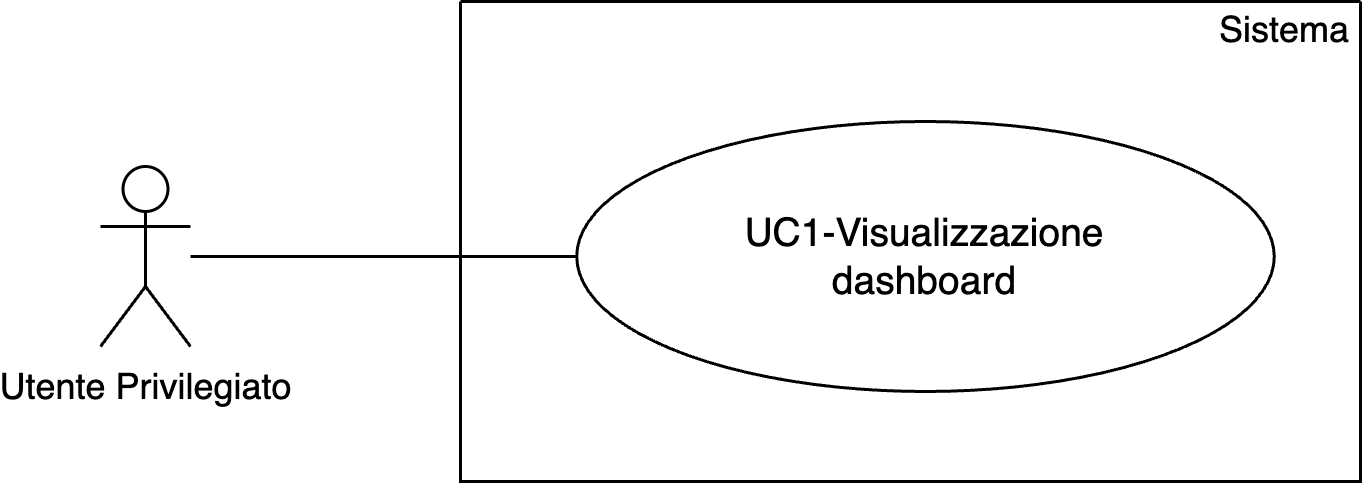
\includegraphics[width=0.7\linewidth]{UC1image.png}
    \caption{UC1 - Visualizzazione Dashboard$_G$}
    \label{fig:UC1}
\end{figure}
\begin{itemize}
    \item \textbf{Attore$_G$ Principale:} Utente privilegiato.
    \item \textbf{Precondizioni:} 
        \begin{itemize}
          \item Il Sistema$_G$ è operativo e accessibile;
        \end{itemize}
    \item \textbf{Postcondizioni:} L'utente privilegiato è in grado di visualizzare una mappa geografica, con i sensori GPS aggiornati in tempo reale (percorsi degli utenti), i vari punti di interesse e le pubblicità offerte agli utenti.
    \item \textbf{Scenario Principale:}
        \begin{enumerate}
            \item L'utente privilegiato accede alla piattaforma di visualizzazione della Dashboard$_G$.
            \item Il Sistema$_G$ mette a disposizione tutte le informazioni storicizzate e ricevute dai sensori, distribuiti su una mappa tramite Marker$_G$.
        \end{enumerate}
    \item \textbf{User-Story$_G$ associata:} Come utente privilegiato, voglio accedere alla Dashboard$_G$ per visualizzare in tempo reale i mezzi che ho messo a noleggio (sensori GPS), i punti di interesse che usufruiscono di questo servizio e le inserzioni che vengono generate per gli utenti che hanno effettuato il noleggio.
\end{itemize}

%%%%%%%%%%%%%%%%%%%%%%%%%%%%%%%%%%%%%%%%%%%%%%%%%%%%%%%%%%%%%%%%%%%%%%%%%%%

\subsubsection{\textbf{UC1.1 - Visualizzazione Percorsi$_G$ sulla mappa}}
\begin{figure}[H]
    \centering
    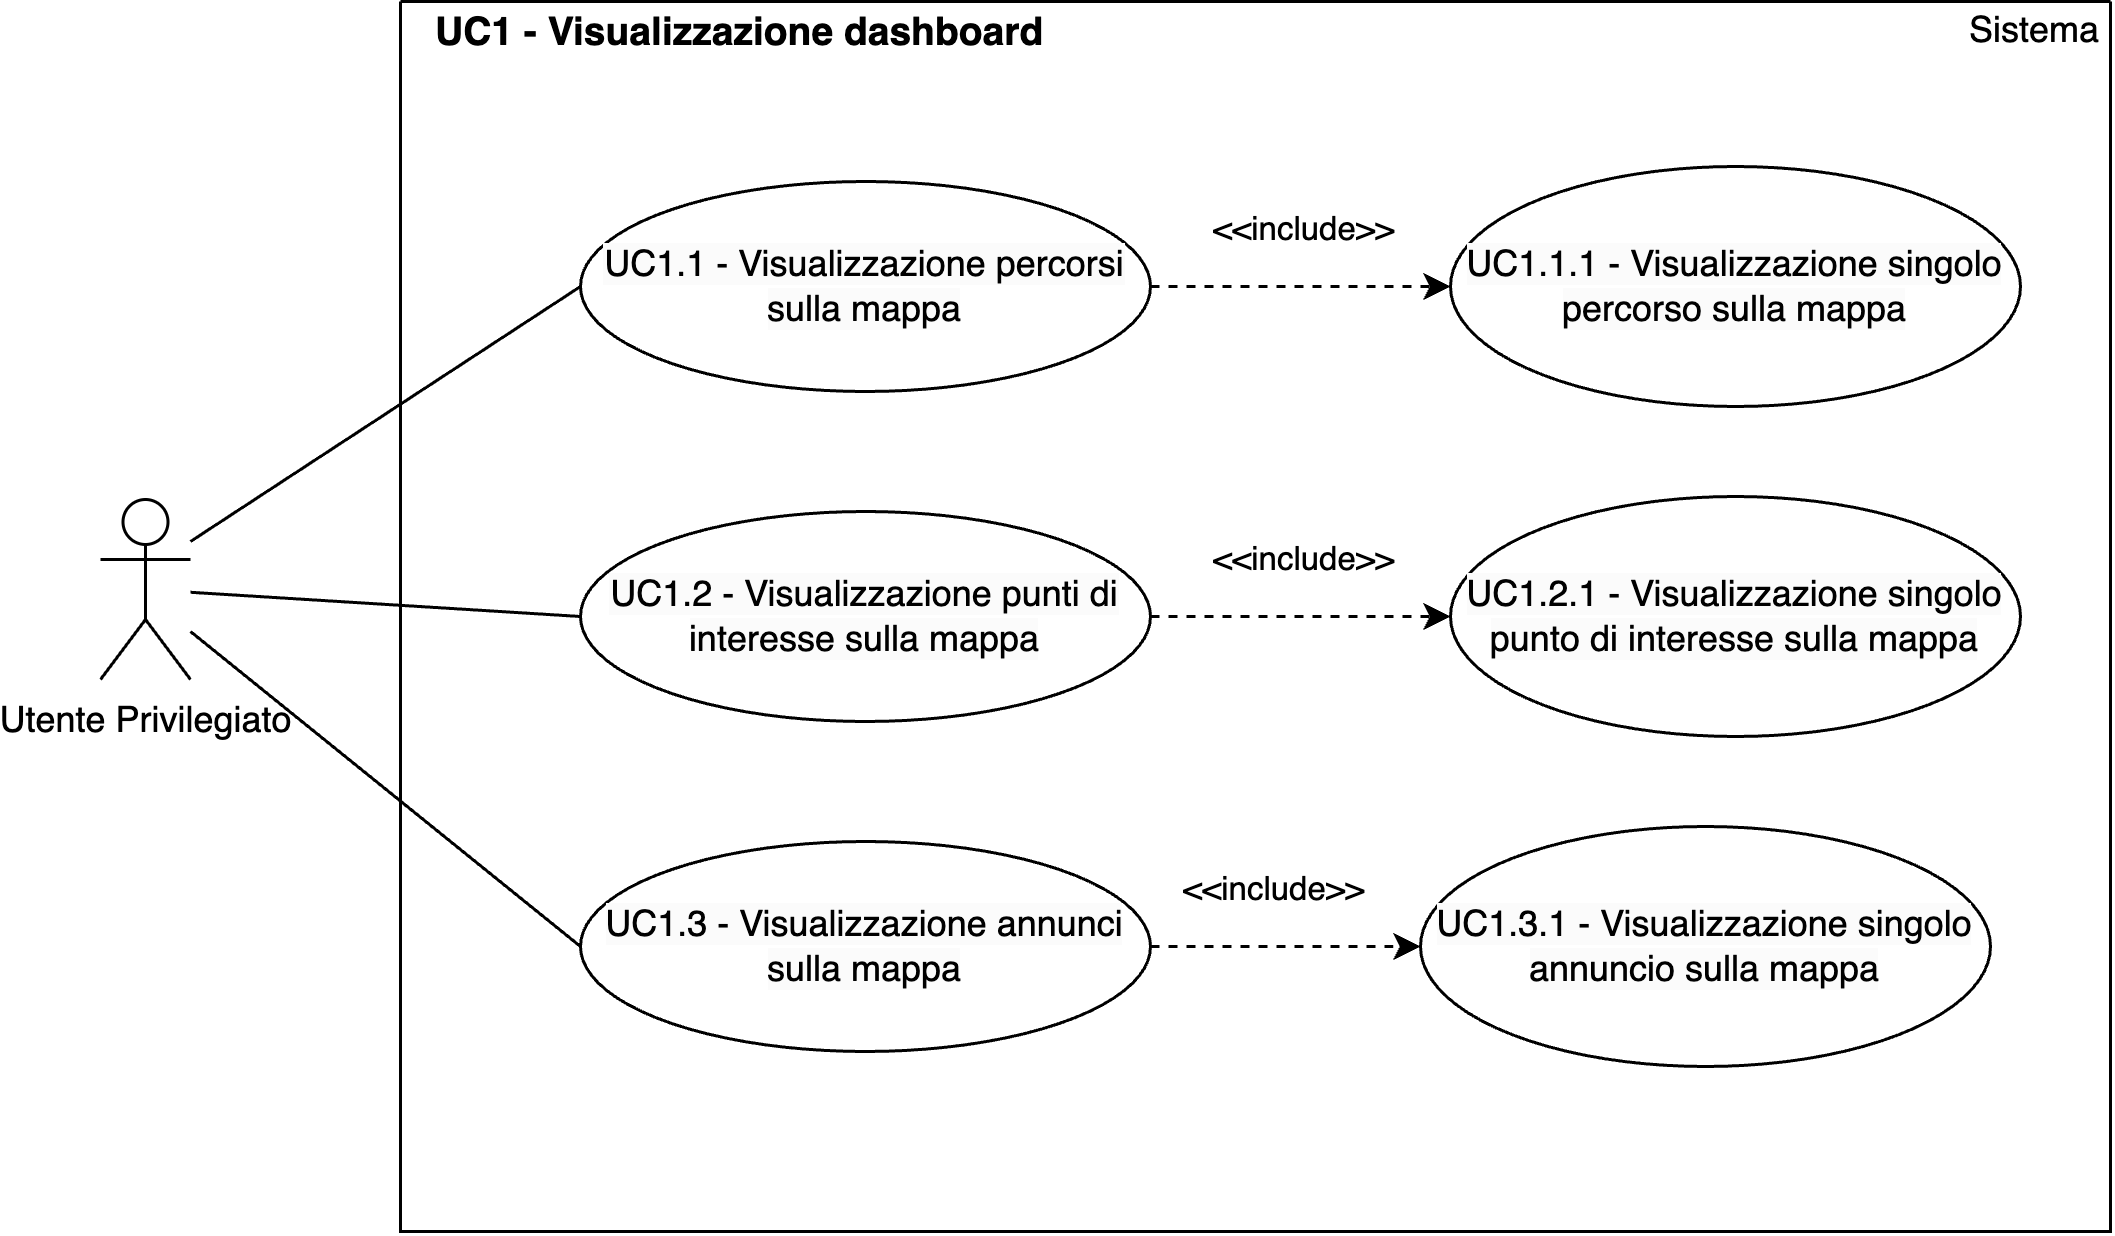
\includegraphics[width=0.7\linewidth]{UC1.123image.png}
    \caption{ UC1.1 -- UC1.2 -- UC1.3 -- UC1.1.1 -- UC1.2.1 -- UC1.3.1}
    \label{fig:UC1.1}
\end{figure}
\label{UC1.1}
\begin{itemize}
     \item \textbf{Attore$_G$ Principale:} Utente Privilegiato.
     \item \textbf{Precondizioni:}
        \begin{itemize}
    		\item L'utente privilegiato sta visualizzando la Dashboard$_G$ (UC1).
        \end{itemize}
     \item \textbf{Postcondizioni:} L'utente privilegiato è in grado di visualizzare i Percorsi$_G$ degli utenti differenziati dai Marker$_G$ presenti sulla mappa.
     \item \textbf{Scenario Principale:}
        \begin{enumerate}
            \item L'utente privilegiato visualizza la Dashboard$_G$ con la mappa interattiva (UC1);
            \item L'utente privilegiato visualizza i Percorsi$_G$ di tutti gli utenti attivi nel Sistema$_G$;
        \end{enumerate}
     \item \textbf{User-Story$_G$ associata:}
     Come utente privilegiato voglio poter visualizzare i vari Percorsi$_G$ effettuati dagli utenti. Questa Dashboard$_G$ permette di tenere traccia dei Percorsi$_G$, tramite dei Marker$_G$ che rappresentano le più recenti posizioni GPS tracciate dal Sistema$_G$.
\end{itemize}
%%%%%%%%%%%%%%%%%%%%%%%%%%%%%%%%%%%%%%%%%%%%%%%%%%%%%%%%%%%%%%%%%%%%%%%%%%%
\subsubsection{\textbf{UC1.2 - Visualizzazione punti di interesse sulla mappa}}
\label{UC1.2}
\begin{itemize}
     \item \textbf{Attore$_G$ Principale:} Utente Privilegiato.
     \item \textbf{Precondizioni:}
        \begin{itemize}
    		\item L'utente privilegiato sta visualizzando la Dashboard$_G$ principale (UC1).
        \end{itemize}
     \item \textbf{Postcondizioni:} L'utente privilegiato è in grado di visualizzare tutti i punti di interesse riconosciuti dal Sistema$_G$ tramite dei Marker$_G$ sulla mappa.
     \item \textbf{Scenario Principale:}
        \begin{enumerate}
            \item L'utente privilegiato visualizza la Dashboard$_G$ con la mappa interattiva (UC1);
            \item Il Sistema$_G$ mette a disposizione tutti i punti di interesse attivi in quel momento.
        \end{enumerate}
     \item \textbf{User-Story$_G$ associata:}
     Come utente privilegiato voglio poter visualizzare tutti i punti di interesse presenti sulla mappa.
\end{itemize}
%%%%%%%%%%%%%%%%%%%%%%%%%%%%%%%%%%%%%%%%%%%%%%%%%%%%%%%%%%%%%%%%%%%%%%%%%%%
\subsubsection{\textbf{UC1.3 - Visualizzazione annunci sulla mappa}}
\label{UC1.3}
\begin{itemize}
    \item \textbf{Attore$_G$ Principale:} Utente Privilegiato.
    \item \textbf{Precondizioni:} 
        \begin{itemize}
    	\item L'utente privilegiato sta visualizzando la Dashboard$_G$ principale (UC1).
        \end{itemize}
     \item \textbf{Postcondizioni:} L'utente privilegiato è in grado di visualizzare gli annunci generati dal Sistema$_G$ tramite dei Marker$_G$ sulla mappa.
    \item \textbf{Scenario Principale:} 
      \begin{enumerate}
      \item L'utente privilegiato visualizza la Dashboard$_G$ con la mappa interattiva (UC1);
            \item Il Sistema$_G$ mette a disposizione tutti gli annunci attivi in quel momento.
	\end{enumerate}
    \item \textbf{User-Story$_G$ associata:} Come utente privilegiato voglio visualizzare sulla mappa gli annunci pubblicitari riservati ai vari utenti.
\end{itemize}
%%%%%%%%%%%%%%%%%%%%%%%%%%%%%%%%%%%%%%%%%%%%%%%%%%%%%%%%%%%%%%%%%%%%%%%%%%%
\subsubsection{\textbf{UC1.1.1 - Visualizzazione singolo Percorso$_G$ sulla mappa}}
\label{UC1.1.1}
\begin{itemize}
     \item \textbf{Attore$_G$ Principale:} Utente Privilegiato.
     \item \textbf{Precondizioni:}
        \begin{itemize}
    		\item L'utente privilegiato sta visualizzando la Dashboard$_G$ (UC1).
    		\item L'utente privilegiato sta visualizzando i Percorsi$_G$ sulla Dashboard$_G$ (UC1.1).
        \end{itemize}
     \item \textbf{Postcondizioni:} L'utente privilegiato è in grado di visualizzare un Marker$_G$ raffigurante la posizione di un singolo utente presente sulla mappa.
     \item \textbf{Scenario Principale:}
        \begin{enumerate}
            \item L'utente privilegiato visualizza la Dashboard$_G$ con la mappa interattiva (UC1);
            \item L'utente privilegiato visualizza i Percorsi$_G$ di tutti gli utenti attivi nel Sistema$_G$(UC1.1);
            \item L'utente privilegiato visualizza un Percorso$_G$ di un utente attivo nel Sistema$_G$.
        \end{enumerate}
     \item \textbf{User-Story$_G$ associata:}
     Come utente privilegiato voglio poter visualizzare un singolo Percorso$_G$ effettuato da un utente. Questa Dashboard$_G$ permette di tenere traccia del singolo Percorso$_G$, tramite un Marker$_G$ che rappresenta la più recente posizione GPS tracciata dal Sistema$_G$.
\end{itemize}
%%%%%%%%%%%%%%%%%%%%%%%%%%%%%%%%%%%%%%%%%%%%%%%%%%%%%%%%%%%%%%%%%%%%%%%%%%%
\subsubsection{\textbf{UC1.2.1 - Visualizzazione singolo punto di interesse sulla mappa}}
\label{UC1.2.1}
\begin{itemize}
     \item \textbf{Attore$_G$ Principale:} Utente Privilegiato.
     \item \textbf{Precondizioni:}
        \begin{itemize}
    		\item L'utente privilegiato sta visualizzando la Dashboard$_G$ (UC1).
    		\item L'utente privilegiato sta visualizzando i punti di interesse sulla Dashboard$_G$ (UC1.2).
        \end{itemize}
     \item \textbf{Postcondizioni:} L'utente privilegiato è in grado di visualizzare un Marker$_G$ raffigurante la posizione di un singolo punto di interesse presente sulla mappa.
     \item \textbf{Scenario Principale:}
        \begin{enumerate}
            \item L'utente privilegiato visualizza la Dashboard$_G$ con la mappa interattiva (UC1);
            \item L'utente privilegiato visualizza tutti i punti di interesse attivi nel Sistema$_G$(UC1.2);
            \item L'utente privilegiato visualizza un punto di interesse attivo nel Sistema$_G$.
        \end{enumerate}
     \item \textbf{User-Story$_G$ associata:}
     Come utente privilegiato voglio poter visualizzare un singolo punto di interesse. Questa Dashboard$_G$ permette di tenere traccia del singolo punto di interesse, tramite un Marker$_G$ che rappresenta la posizione GPS salvata nel Sistema$_G$.
\end{itemize}
%%%%%%%%%%%%%%%%%%%%%%%%%%%%%%%%%%%%%%%%%%%%%%%%%%%%%%%%%%%%%%%%%%%%%%%%%%%
\subsubsection{\textbf{UC1.3.1 - Visualizzazione singolo annuncio sulla mappa}}
\label{UC1.3.1}
\begin{itemize}
     \item \textbf{Attore$_G$ Principale:} Utente Privilegiato.
     \item \textbf{Precondizioni:}
        \begin{itemize}
        \item Il Sistema$_G$ è operativo e accessibile.
    	\item L'utente privilegiato sta visualizzando la Dashboard$_G$ (UC1).
    	\item L'utente privilegiato sta visualizzando gli annunci sulla Dashboard$_G$ (UC1.3).
        \end{itemize}
     \item \textbf{Postcondizioni:} L'utente privilegiato è in grado di visualizzare un Marker$_G$ raffigurante un singolo annuncio presente sulla mappa.
     \item \textbf{Scenario Principale:}
        \begin{enumerate}
            \item L'utente privilegiato visualizza la Dashboard$_G$ con la mappa interattiva (UC1);
            \item L'utente privilegiato visualizza gli annunci attivi nel Sistema$_G$(UC1.3);
            \item L'utente privilegiato visualizza un annuncio attivo nel Sistema$_G$.
        \end{enumerate}
     \item \textbf{User-Story$_G$ associata:}
     Come utente privilegiato voglio poter visualizzare un singolo annuncio generato dal Sistema$_G$. Questa Dashboard$_G$ permette di tenere traccia del singolo annuncio, tramite un Marker$_G$ che rappresenta la posizione in cui l'utente e il punto di interesse coinvolti sono presenti.
\end{itemize}
%%%%%%%%%%%%%%%%%%%%%%%%%%%%%%%%%%%%%%%%%%%%%%%%%%%%%%%%%%%%%%%%%%%%%%%%%%%
\subsubsection{\textbf{UC2 - Visualizzazione annuncio}}
\begin{figure}[H]
    \centering
    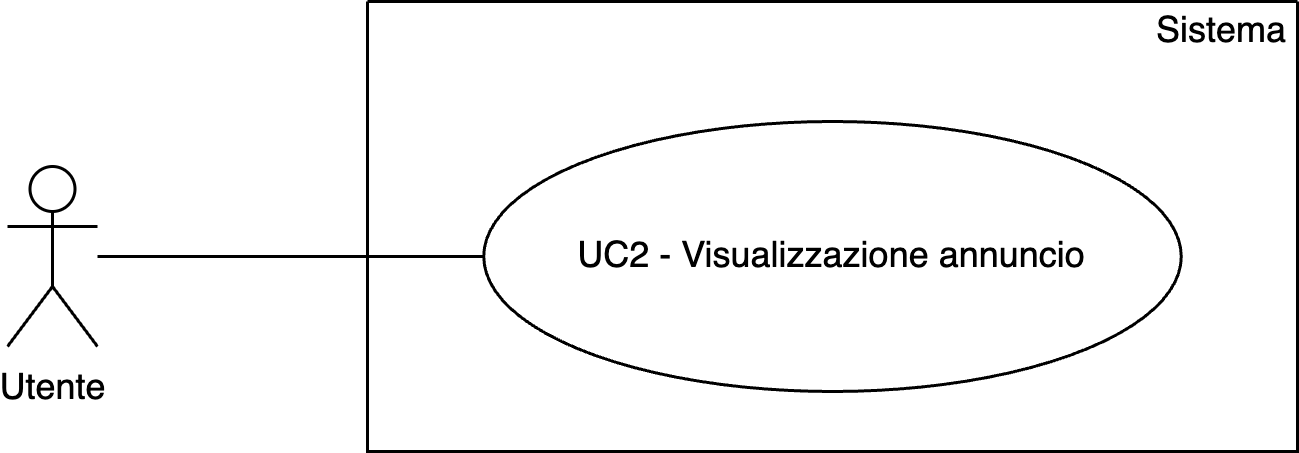
\includegraphics[width=0.7\linewidth]{UC2image.png}
    \caption{UC2 - Visualizzazione annuncio}
    \label{fig:UC2}
\end{figure}
\begin{itemize}
    \item \textbf{Attore$_G$ Principale:} Utente.
    \item \textbf{Precondizioni:} 
        \begin{itemize}
    	\item Il Sistema$_G$ è operativo e accessibile;
    	\item Un utente entra nell'area di un punto di interesse.
        \end{itemize}
    \item \textbf{Postcondizioni:} L'Utente visualizzerà un messaggio contenente un annuncio personalizzato in base ai suoi dati personali e al punto di interesse.
    \item \textbf{Scenario Principale:} 
        \begin{enumerate}
            \item Un utente, mentre si muove sulla mappa, passa nell'area di un punto di interesse;
            \item Il Sistema$_G$ elabora le informazioni dell'utente e del punto di interesse per generare il testo dell'eventuale annuncio;
            \item Il Sistema$_G$ invia all'utente il messaggio contenente l'annuncio se questo è stato generato. L'annuncio contiene come informazioni almeno il nome del punto di interesse e il suo indirizzo.
            % Da considerare l'idea di suddividere l'UC mediante include per ciascuna delle informazioni contenute nell'annuncio
        \end{enumerate}
    \item \textbf{User-Story$_G$ associata:} Come utente voglio visualizzare gli annunci pubblicitari personalizzati che mi arrivano, contenenti sicuramente almeno nome e indirizzo del punto di interesse oggetto dell'annuncio.
\end{itemize}
%%%%%%%%%%%%%%%%%%%%%%%%%%%%%%%%%%%%%%%%%%%%%%%%%%%%%%%%%%%%%%%%%%%%%%%%%%%
\subsubsection{\textbf{UC3 - Visualizzazione mappa singolo utente}}
\begin{figure}[H]
    \centering
    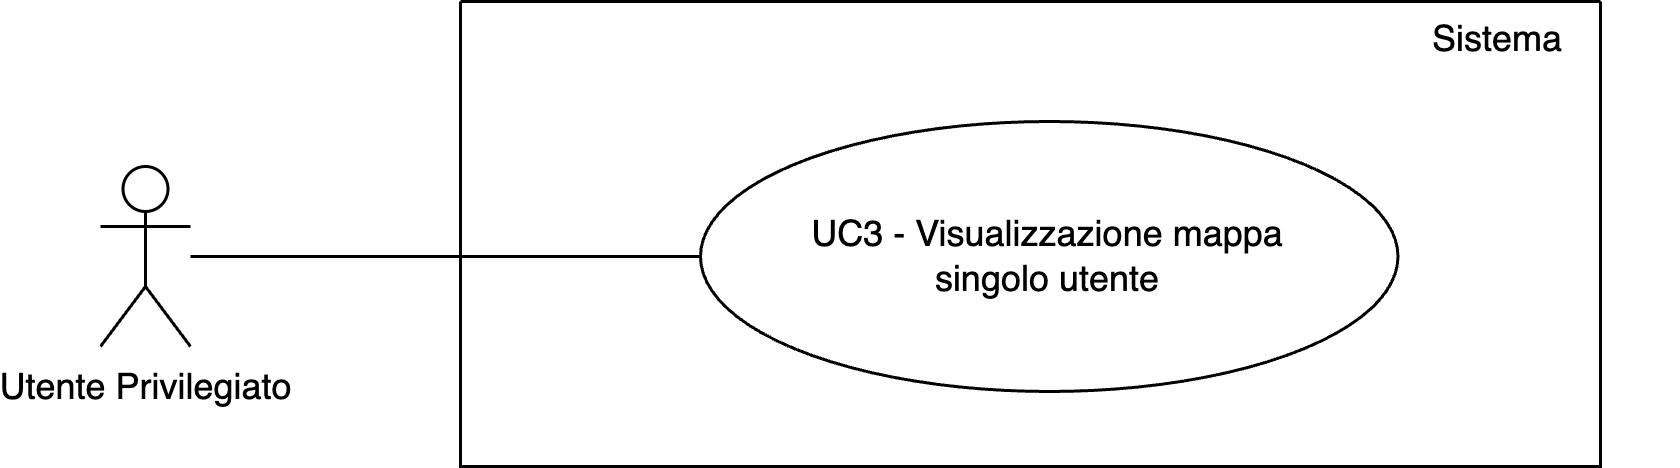
\includegraphics[width=0.7\linewidth]{UC3image.png}
    \caption{UC3 - Visualizzazione mappa singolo utente}
    \label{fig:UC3}
\end{figure}
    \label{UC3}
\begin{itemize}
     \item \textbf{Attore$_G$ Principale:} Utente Privilegiato.
     \item \textbf{Precondizioni:}
        \begin{itemize}
    		\item L'utente privilegiato sta visualizzando la Dashboard$_G$ (UC1);
    	        \item L'utente privilegiato sta visualizzando i Percorsi$_G$ presenti sulla mappa (UC1.1);
    	        \item L'utente privilegiato ha selezionato un Marker$_G$, riferito ad un singolo utente (UC1.1.1).
        \end{itemize}
     \item \textbf{Postcondizioni:} L'utente privilegiato è in grado di ottenere informazioni più dettagliate del Marker$_G$ selezionato tramite una Dashboard$_G$ apposita.
     \item \textbf{Scenario Principale:}
        \begin{enumerate}
            \item L'utente privilegiato visualizza la Dashboard$_G$ con la mappa interattiva (UC1);
            \item L'utente privilegiato seleziona un Marker$_G$ di un determinato Percorso$_G$ (UC1.1.1) per visualizzarne la Dashboard$_G$ specifica;
            \item Il Sistema$_G$ mette a disposizione lo storico delle posizioni e dei messaggi archiviati per quel Marker$_G$.
        \end{enumerate}
     \item \textbf{User-Story$_G$ associata:}
     Come utente privilegiato voglio selezionare i vari Marker$_G$, che indicano i mezzi di trasporto, presenti sulla mappa dei Percorsi$_G$, in modo da visualizzare una Dashboard$_G$ contenente le informazioni relative ad un singolo utente. Questa Dashboard$_G$ permette di visualizzare i dettagli sullo storico completo delle posizioni e sull'utente che sta utilizzando il mezzo. Inoltre permette di poter vedere tutti gli annunci inviati a quell'utente durante la stessa giornata.
\end{itemize}

%%%%%%%%%%%%%%%%%%%%%%%%%%%%%%%%%%%%%%%%%%%%%%%%%%%%%%%%%%%%%%%%%%%%%%%%%%%

\subsubsection{\textbf{UC3.1 - Visualizzazione storico posizioni GPS}}
\begin{figure}[H]
    \centering
    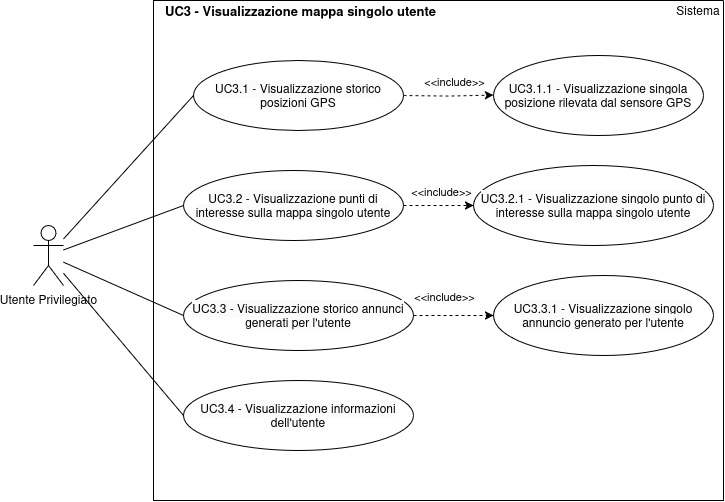
\includegraphics[width=0.7\linewidth]{UC3.1234image.png}
    \caption{ UC3.1 -- UC3.2 -- UC3.3 -- UC3.4 -- UC3.1.1 -- UC3.2.1 -- UC3.3.1}
    \label{fig:UC3.1}
\end{figure}
\label{UC3.1}
\begin{itemize}
     \item \textbf{Attore$_G$ Principale:} Utente Privilegiato.
     \item \textbf{Precondizioni:}
        \begin{itemize}
    		\item L'utente privilegiato sta visualizzando la Dashboard$_G$ singolo utente (UC3).
        \end{itemize}
     \item \textbf{Postcondizioni:} L'utente privilegiato è in grado di visualizzare lo storico delle posizioni dell'utente differenziati da Marker$_G$ presenti sulla mappa.
     \item \textbf{Scenario Principale:}
        \begin{enumerate}
            \item L'utente privilegiato visualizza la Dashboard$_G$ con la mappa interattiva (UC1);
            \item L'utente privilegiato seleziona un Marker$_G$ di un determinato Percorso$_G$ (UC1.1.1) per visualizzarne la Dashboard$_G$ specifica (UC3);
            \item Il Sistema$_G$ mette a disposizione lo storico delle posizioni, distinte da Marker$_G$, per l'utente selezionato.
        \end{enumerate}
     \item \textbf{User-Story$_G$ associata:}
     Come utente privilegiato voglio poter visualizzare lo storico delle posizioni di un utente. Questa Dashboard$_G$ permette di tenere traccia delle posizioni di un singolo utente tramite dei Marker$_G$.
\end{itemize}
%%%%%%%%%%%%%%%%%%%%%%%%%%%%%%%%%%%%%%%%%%%%%%%%%%%%%%%%%%%%%%%%%%%%%%%%%%%
\subsubsection{\textbf{UC3.2 - Visualizzazione punti di interesse sulla mappa singolo utente}}
\label{UC3.2}
\begin{itemize}
     \item \textbf{Attore$_G$ Principale:} Utente Privilegiato.
     \item \textbf{Precondizioni:}
        \begin{itemize}
    		\item L'utente privilegiato sta visualizzando la Dashboard$_G$ singolo utente (UC3).
        \end{itemize}
     \item \textbf{Postcondizioni:} L'utente privilegiato è in grado di visualizzare tutti i punti di interesse riconosciuti dal Sistema$_G$ tramite dei Marker$_G$ sulla mappa.
     \item \textbf{Scenario Principale:}
        \begin{enumerate}
            \item L'utente privilegiato visualizza la Dashboard$_G$ con la mappa interattiva (UC1);
            \item L'utente privilegiato seleziona un Marker$_G$ di un determinato Percorso$_G$ (UC1.1.1) per visualizzarne la Dashboard$_G$ specifica (UC3);
            \item Il Sistema$_G$ mette a disposizione tutti i punti di interesse attivi in quel momento.
        \end{enumerate}
     \item \textbf{User-Story$_G$ associata:}
     Come utente privilegiato voglio poter visualizzare tutti i punti di interesse presenti sulla mappa.
\end{itemize}
%%%%%%%%%%%%%%%%%%%%%%%%%%%%%%%%%%%%%%%%%%%%%%%%%%%%%%%%%%%%%%%%%%%%%%%%%%%
\subsubsection{\textbf{UC3.3 - Visualizzazione storico annunci generati per l'utente}}
\label{UC3.3}
\begin{itemize}
    \item \textbf{Attore$_G$ Principale:} Utente Privilegiato.
    \item \textbf{Precondizioni:} 
        \begin{itemize}
    		\item L'utente privilegiato sta visualizzando la Dashboard$_G$ singolo utente (UC3).
        \end{itemize}
     \item \textbf{Postcondizioni:} L'utente privilegiato è in grado di visualizzare lo storico degli annunci generati dal Sistema$_G$ per l'utente tramite dei Marker$_G$ sulla mappa.
    \item \textbf{Scenario Principale:} 
      \begin{enumerate}
            \item L'utente privilegiato visualizza la Dashboard$_G$ con la mappa interattiva (UC1);
            \item L'utente privilegiato seleziona un Marker$_G$ di un determinato Percorso$_G$ (UC1.1.1) per visualizzarne la Dashboard$_G$ specifica (UC3);
            \item Il Sistema$_G$ mette a disposizione lo storico di tutti gli annunci generati, distinti da Marker$_G$, per l'utente selezionato.
	\end{enumerate}
    \item \textbf{User-Story$_G$ associata:} Come utente privilegiato voglio visualizzare sulla mappa lo storico degli annunci pubblicitari generati per l'utente selezionato.
\end{itemize}
%%%%%%%%%%%%%%%%%%%%%%%%%%%%%%%%%%%%%%%%%%%%%%%%%%%%%%%%%%%%%%%%%%%%%%%%%%%
\subsubsection{\textbf{UC3.4 - Visualizzazione informazioni dell'utente}}
\label{UC3.4}
\begin{itemize}
     \item \textbf{Attore$_G$ Principale:} Utente Privilegiato.
     \item \textbf{Precondizioni:}
        \begin{itemize}
    		\item L'utente privilegiato sta visualizzando la Dashboard$_G$ singolo utente (UC3).
        \end{itemize}
      \item \textbf{Postcondizioni:} L'utente privilegiato visualizza un pannello contenente le informazioni dell'utente, precedentemente selezionato, in forma tabellare. 
      \item \textbf{Scenario Principale:}
        \begin{enumerate}
            \item L'utente privilegiato ha accesso alla Dashboard$_G$ di un singolo utente(UC3);
            \item Il Sistema$_G$ riporta  in un pannello apposito le informazioni dell'utente in forma tabellare;
            \item La tabella conterrà i dati dell'utente che sta utilizzando il mezzo. I dati dell'utente presenti in tabella saranno:
              \begin{itemize}
              \item Nome;
              \item Cognome;
              \item Email;
              \item Genere;
              \item Data di nascita;
              \item Stato civile.
              \end{itemize}
        \end{enumerate}
     \item \textbf{User-Story$_G$ associata:}
       Come utente privilegiato voglio visualizzare, in un pannello dedicato, le informazioni di un singolo utente in forma tabellare.
\end{itemize}

%%%%%%%%%%%%%%%%%%%%%%%%%%%%%%%%%%%%%%%%%%%%%%%%%%%%%%%%%%%%%%%%%%%%%%%%%%%
\subsubsection{\textbf{UC3.1.1 - Visualizzazione singola posizione rilevata dal sensore GPS}}
\label{UC3.1.1}
\begin{itemize}
     \item \textbf{Attore$_G$ Principale:} Utente Privilegiato.
     \item \textbf{Precondizioni:}
        \begin{itemize}
    		\item L'utente privilegiato sta visualizzando la Dashboard$_G$ singolo utente (UC3);
    		\item L'utente privilegiato sta visualizzando lo storico delle posizioni sulla Dashboard$_G$ singolo utente (UC3.1).
        \end{itemize}
     \item \textbf{Postcondizioni:} L'utente privilegiato è in grado di visualizzare sulla mappa un Marker$_G$ raffigurante la posizione dell'utente in un determinato istante.
     \item \textbf{Scenario Principale:}
        \begin{enumerate}
            \item L'utente privilegiato visualizza la Dashboard$_G$ con la mappa interattiva (UC1);
            \item L'utente privilegiato seleziona un Marker$_G$ di un determinato Percorso$_G$ (UC1.1.1) per visualizzarne la Dashboard$_G$ specifica (UC3);
            \item L'utente privilegiato visualizza lo storico delle posizioni, distinte da Marker$_G$, per l'utente selezionato (UC3.1);
            \item L'utente privilegiato visualizza nella mappa la posizione dell'utente in un determinato istante, tramite un Marker$_G$.
        \end{enumerate}
     \item \textbf{User-Story$_G$ associata:}
     Come utente privilegiato voglio poter visualizzare una singola posizione di un utente rilevata dal sensore GPS. Questa Dashboard$_G$ permette di tenere traccia delle singole posizioni di un utente tramite un Marker$_G$.
\end{itemize}
%%%%%%%%%%%%%%%%%%%%%%%%%%%%%%%%%%%%%%%%%%%%%%%%%%%%%%%%%%%%%%%%%%%%%%%%%%%
\subsubsection{\textbf{UC3.2.1 - Visualizzazione singolo punto di interesse sulla mappa}}
\label{UC3.2.1}
\begin{itemize}
     \item \textbf{Attore$_G$ Principale:} Utente Privilegiato.
     \item \textbf{Precondizioni:}
        \begin{itemize}
    		\item L'utente privilegiato sta visualizzando la Dashboard$_G$ singolo utente (UC3);
    		\item L'utente privilegiato sta visualizzando i punti di interesse sulla Dashboard$_G$ singolo utente (UC3.2).
        \end{itemize}
     \item \textbf{Postcondizioni:} L'utente privilegiato è in grado di visualizzare un Marker$_G$ raffigurante la posizione di un singolo punto di interesse presente sulla mappa singolo utente.
     \item \textbf{Scenario Principale:}
        \begin{enumerate}
            \item L'utente privilegiato visualizza la Dashboard$_G$ con la mappa interattiva (UC1);
            \item L'utente privilegiato seleziona un Marker$_G$ di un determinato Percorso$_G$ (UC1.1.1) per visualizzarne la Dashboard$_G$ specifica (UC3);
            \item L'utente privilegiato visualizza tutti i punti di interesse attivi nel Sistema$_G$(UC3.2);
            \item L'utente privilegiato visualizza un punto di interesse attivo nel Sistema$_G$.
        \end{enumerate}
     \item \textbf{User-Story$_G$ associata:}
     Come utente privilegiato voglio poter visualizzare un singolo punto di interesse. Questa Dashboard$_G$ permette di tenere traccia del singolo punto di interesse, tramite un Marker$_G$ che rappresenta la posizione GPS salvata nel Sistema$_G$.
\end{itemize}
%%%%%%%%%%%%%%%%%%%%%%%%%%%%%%%%%%%%%%%%%%%%%%%%%%%%%%%%%%%%%%%%%%%%%%%%%%%
\subsubsection{\textbf{UC3.3.1 - Visualizzazione singolo annuncio generato per l'utente}}
\label{UC3.3.1}
\begin{itemize}
     \item \textbf{Attore$_G$ Principale:} Utente Privilegiato.
     \item \textbf{Precondizioni:}
        \begin{itemize}
    		\item L'utente privilegiato sta visualizzando la Dashboard$_G$ singolo utente (UC3);
    		\item L'utente privilegiato sta visualizzando lo storico degli annunci generati per l'utente sulla Dashboard$_G$ singolo utente (UC3.3).
        \end{itemize}
     \item \textbf{Postcondizioni:} L'utente privilegiato è in grado di visualizzare un Marker$_G$ raffigurante un singolo annuncio generato per l'utente presente sulla mappa.
     \item \textbf{Scenario Principale:}
        \begin{enumerate}
            \item L'utente privilegiato visualizza la Dashboard$_G$ con la mappa interattiva (UC1);
            \item L'utente privilegiato seleziona un Marker$_G$ di un determinato Percorso$_G$ (UC1.1.1) per visualizzarne la Dashboard$_G$ specifica (UC3);
            \item L'utente privilegiato visualizza lo storico degli annunci, distinti da Marker$_G$, generati dal Sistema$_G$ per l'utente selezionato (UC3.3);
            \item L'utente privilegiato visualizza nella mappa, tramite un Marker$_G$, un annuncio generato per l'utente.
        \end{enumerate}
     \item \textbf{User-Story$_G$ associata:}
     Come utente privilegiato voglio poter visualizzare un singolo annuncio generato dal Sistema$_G$ per l'utente. Questa Dashboard$_G$ permette di tenere traccia del singolo annuncio, tramite un Marker$_G$ che rappresenta la posizione in cui l'utente e il punto di interesse coinvolti erano presenti.
\end{itemize}

%%%%%%%%%%%%%%%%%%%%%%%%%%%%%%%%%%%%%%%%%%%%%%%%%%%%%%%%%%%%%%%%%%%%%%%%%%%
\subsubsection{\textbf{UC3.4.1 - Visualizzazione nome dell'utente}}
\begin{figure}[H]
    \centering
    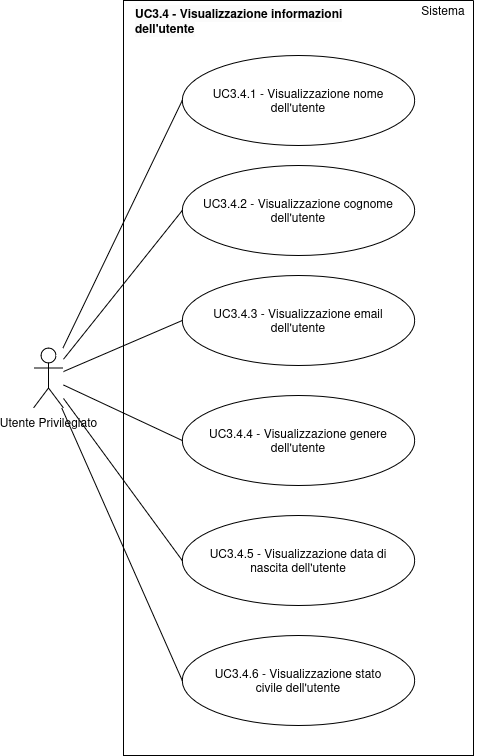
\includegraphics[width=0.7\linewidth]{UC3.4.1image.png}
    \caption{UC3.4.1 -- UC3.4.2 -- UC3.4.3 -- UC3.4.4 -- UC3.4.5 -- UC3.4.6}
    \label{fig:UC3.4.1}
\end{figure}
\label{UC3.4.1}
\begin{itemize}
     \item \textbf{Attore$_G$ Principale:} Utente Privilegiato.
     \item \textbf{Precondizioni:}
        \begin{itemize}
    	\item L'utente privilegiato sta visualizzando la Dashboard$_G$ singolo utente (UC3).
          \item L'utente privilegiato sta visualizzando un pannello contenente le informazioni dell'utente in forma tabellare (UC3.4).
        \end{itemize}
      \item \textbf{Postcondizioni:} L'utente privilegiato visualizza il nome dell'utente. 
      \item \textbf{Scenario Principale:}
        \begin{enumerate}
            \item L'utente privilegiato ha accesso alla Dashboard$_G$ di un singolo utente(UC3);
            \item Il Sistema$_G$ riporta  in un pannello apposito le informazioni dell'utente in forma tabellare (UC3.4);
            \item La tabella conterrà il nome dell'utente.
        \end{enumerate}
     \item \textbf{User-Story$_G$ associata:}
       Come utente privilegiato voglio visualizzare il nome dell'utente.
\end{itemize}

%%%%%%%%%%%%%%%%%%%%%%%%%%%%%%%%%%%%%%%%%%%%%%%%%%%%%%%%%%%%%%%%%%%%%%%%%%%
\subsubsection{\textbf{UC3.4.2 - Visualizzazione cognome dell'utente}}
\label{UC3.4.2}
\begin{itemize}
     \item \textbf{Attore$_G$ Principale:} Utente Privilegiato.
     \item \textbf{Precondizioni:}
        \begin{itemize}
    	\item L'utente privilegiato sta visualizzando la Dashboard$_G$ singolo utente (UC3).
          \item L'utente privilegiato sta visualizzando un pannello contenente le informazioni dell'utente in forma tabellare (UC3.4).
        \end{itemize}
      \item \textbf{Postcondizioni:} L'utente privilegiato visualizza il cognome dell'utente. 
      \item \textbf{Scenario Principale:}
        \begin{enumerate}
            \item L'utente privilegiato ha accesso alla Dashboard$_G$ di un singolo utente(UC3);
            \item Il Sistema$_G$ riporta  in un pannello apposito le informazioni dell'utente in forma tabellare (UC3.4);
            \item La tabella conterrà il cognome dell'utente.
        \end{enumerate}
     \item \textbf{User-Story$_G$ associata:}
       Come utente privilegiato voglio visualizzare il cognome dell'utente.
\end{itemize}

%%%%%%%%%%%%%%%%%%%%%%%%%%%%%%%%%%%%%%%%%%%%%%%%%%%%%%%%%%%%%%%%%%%%%%%%%%%
\subsubsection{\textbf{UC3.4.3 - Visualizzazione email dell'utente}}
\label{UC3.4.3}
\begin{itemize}
     \item \textbf{Attore$_G$ Principale:} Utente Privilegiato.
     \item \textbf{Precondizioni:}
        \begin{itemize}
    	\item L'utente privilegiato sta visualizzando la Dashboard$_G$ singolo utente (UC3).
          \item L'utente privilegiato sta visualizzando un pannello contenente le informazioni dell'utente in forma tabellare (UC3.4).
        \end{itemize}
      \item \textbf{Postcondizioni:} L'utente privilegiato visualizza l'email dell'utente.
      \item \textbf{Scenario Principale:}
        \begin{enumerate}
            \item L'utente privilegiato ha accesso alla Dashboard$_G$ di un singolo utente(UC3);
            \item Il Sistema$_G$ riporta  in un pannello apposito le informazioni dell'utente in forma tabellare (UC3.4);
            \item La tabella conterrà l'email dell'utente.
        \end{enumerate}
     \item \textbf{User-Story$_G$ associata:}
       Come utente privilegiato voglio visualizzare l'email dell'utente.
\end{itemize}

%%%%%%%%%%%%%%%%%%%%%%%%%%%%%%%%%%%%%%%%%%%%%%%%%%%%%%%%%%%%%%%%%%%%%%%%%%%
\subsubsection{\textbf{UC3.4.4 - Visualizzazione genere dell'utente}}
\label{UC3.4.4}
\begin{itemize}
     \item \textbf{Attore$_G$ Principale:} Utente Privilegiato.
     \item \textbf{Precondizioni:}
        \begin{itemize}
    	\item L'utente privilegiato sta visualizzando la Dashboard$_G$ singolo utente (UC3).
          \item L'utente privilegiato sta visualizzando un pannello contenente le informazioni dell'utente in forma tabellare (UC3.4).
        \end{itemize}
      \item \textbf{Postcondizioni:} L'utente privilegiato visualizza il genere dell'utente.
      \item \textbf{Scenario Principale:}
        \begin{enumerate}
            \item L'utente privilegiato ha accesso alla Dashboard$_G$ di un singolo utente(UC3);
            \item Il Sistema$_G$ riporta  in un pannello apposito le informazioni dell'utente in forma tabellare (UC3.4);
            \item La tabella conterrà il genere dell'utente.
        \end{enumerate}
     \item \textbf{User-Story$_G$ associata:}
       Come utente privilegiato voglio visualizzare il genere dell'utente.
\end{itemize}

%%%%%%%%%%%%%%%%%%%%%%%%%%%%%%%%%%%%%%%%%%%%%%%%%%%%%%%%%%%%%%%%%%%%%%%%%%%
\subsubsection{\textbf{UC3.4.5 - Visualizzazione data di nascita dell'utente}}
\label{UC3.4.5}
\begin{itemize}
     \item \textbf{Attore$_G$ Principale:} Utente Privilegiato.
     \item \textbf{Precondizioni:}
        \begin{itemize}
    	\item L'utente privilegiato sta visualizzando la Dashboard$_G$ singolo utente (UC3).
          \item L'utente privilegiato sta visualizzando un pannello contenente le informazioni dell'utente in forma tabellare (UC3.4).
        \end{itemize}
      \item \textbf{Postcondizioni:} L'utente privilegiato visualizza la data di nascita dell'utente. 
      \item \textbf{Scenario Principale:}
        \begin{enumerate}
            \item L'utente privilegiato ha accesso alla Dashboard$_G$ di un singolo utente(UC3);
            \item Il Sistema$_G$ riporta  in un pannello apposito le informazioni dell'utente in forma tabellare (UC3.4);
            \item La tabella conterrà la data di nascita dell'utente.
        \end{enumerate}
     \item \textbf{User-Story$_G$ associata:}
       Come utente privilegiato voglio visualizzare la data di nascita dell'utente.
\end{itemize}

%%%%%%%%%%%%%%%%%%%%%%%%%%%%%%%%%%%%%%%%%%%%%%%%%%%%%%%%%%%%%%%%%%%%%%%%%%%
\subsubsection{\textbf{UC3.4.6- Visualizzazione stato civile dell'utente}}
\label{UC3.4.6}
\begin{itemize}
     \item \textbf{Attore$_G$ Principale:} Utente Privilegiato.
     \item \textbf{Precondizioni:}
        \begin{itemize}
    	\item L'utente privilegiato sta visualizzando la Dashboard$_G$ singolo utente (UC3).
          \item L'utente privilegiato sta visualizzando un pannello contenente le informazioni dell'utente in forma tabellare (UC3.4).
        \end{itemize}
      \item \textbf{Postcondizioni:} L'utente privilegiato visualizza lo stato civile dell'utente. 
      \item \textbf{Scenario Principale:}
        \begin{enumerate}
            \item L'utente privilegiato ha accesso alla Dashboard$_G$ di un singolo utente(UC3);
            \item Il Sistema$_G$ riporta  in un pannello apposito le informazioni dell'utente in forma tabellare (UC3.4);
            \item La tabella conterrà lo stato civile dell'utente.
        \end{enumerate}
     \item \textbf{User-Story$_G$ associata:}
       Come utente privilegiato voglio visualizzare lo stato civile dell'utente.
\end{itemize}

%%%%%%%%%%%%%%%%%%%%%%%%%%%%%%%%%%%%%%%%%%%%%%%%%%%%%%%%%%%%%%%%%%%%%%%%%%%
\subsubsection{\textbf{UC4 - Visualizzazione dettagli dei Marker$_G$ utente sulla mappa}}
\begin{figure}[H]
    \centering
    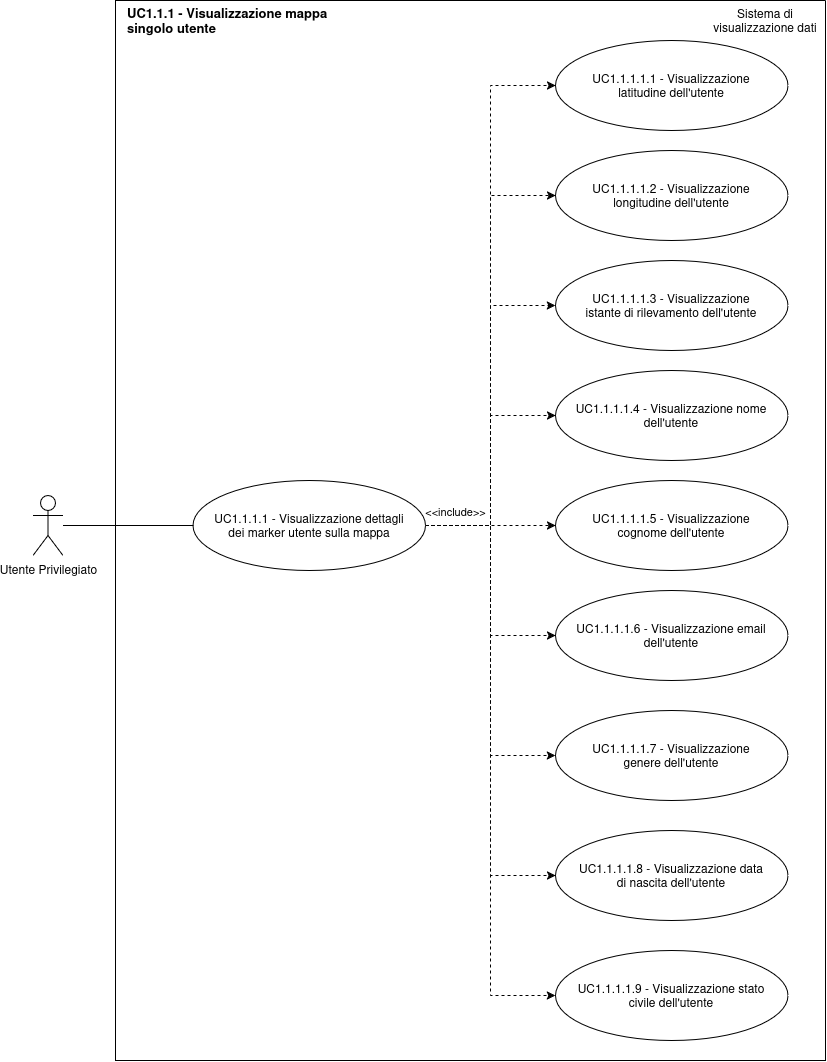
\includegraphics[width=0.7\linewidth]{UC4image.png}
    \caption{UC4 -- UC4.1 -- UC4.2 -- UC4.3}
    \label{fig:UC4}
\end{figure}
\label{UC4}
\begin{itemize}
     \item \textbf{Attore$_G$ Principale:} Utente Privilegiato.
     \item \textbf{Precondizioni:}
        \begin{itemize}
    		\item L'utente privilegiato sta visualizzando la Dashboard$_G$ singolo utente (UC3);
    		\item L'utente privilegiato sta visualizzando lo storico delle posizioni sulla Dashboard$_G$ singolo utente (UC3.1).
          \item L'utente privilegiato ha selezionato un Marker$_G$, raffigurante la posizione dell'utente ad un determinato istante, presente nella mappa di singolo utente.
        \end{itemize}
      \item \textbf{Postcondizioni:} L'utente privilegiato visualizza un pannello contenente le informazioni del Marker$_G$ utente selezionato in forma tabellare. 
      \item \textbf{Scenario Principale:}
        \begin{enumerate}
            \item L'utente privilegiato ha accesso alla Dashboard$_G$ di un singolo utente(UC3);
            \item L'utente privilegiato seleziona un Marker$_G$ utente presente sulla mappa di un singolo utente;
            \item Il Sistema$_G$ riporta le informazioni del Marker$_G$ in forma tabellare.
            \item La tabella conterrà la posizione, espressa in latitudine e longitudine e l'istante di rilevamento.
        \end{enumerate}
     \item \textbf{User-Story$_G$ associata:}
       Come utente privilegiato voglio selezionare un Marker$_G$, che indica la posizione dell'utente, presente sulla mappa di singolo utente, per poter visualizzare le informazioni specifiche del Marker$_G$ selezionato.
\end{itemize}

%%%%%%%%%%%%%%%%%%%%%%%%%%%%%%%%%%%%%%%%%%%%%%%%%%%%%%%%%%%%%%%%%%%%%%%%%%%
\subsubsection{\textbf{UC4.1 - Visualizzazione latitudine dell'utente}}
\label{UC4.1}
\begin{itemize}
     \item \textbf{Attore$_G$ Principale:} Utente Privilegiato.
     \item \textbf{Precondizioni:}
        \begin{itemize}
          \item L'utente privilegiato ha selezionato un Marker$_G$ utente (UC3.1.1) presente nella mappa di singolo utente (UC3);
          \item L'utente privilegiato sta visualizzando un pannello contenente la tabella delle informazioni del Marker$_G$ utente selezionato (UC4).
        \end{itemize}
      \item \textbf{Postcondizioni:} L'utente privilegiato visualizza la latitudine rispettiva al Marker$_G$ utente selezionato. 
      \item \textbf{Scenario Principale:}
        \begin{enumerate}
            \item L'utente privilegiato ha accesso alla Dashboard$_G$ di un singolo utente(UC3);
            \item L'utente privilegiato seleziona un Marker$_G$ utente presente sulla mappa di un singolo utente;
            \item Il Sistema$_G$ riporta le informazioni del Marker$_G$ in forma tabellare (UC4);
            \item La tabella conterrà la latitudine del Marker$_G$ utente selezionato.
        \end{enumerate}
     \item \textbf{User-Story$_G$ associata:}
       Come utente privilegiato voglio visualizzare la latitudine del Marker$_G$ selezionato.
\end{itemize}

%%%%%%%%%%%%%%%%%%%%%%%%%%%%%%%%%%%%%%%%%%%%%%%%%%%%%%%%%%%%%%%%%%%%%%%%%%%
\subsubsection{\textbf{UC4.2 - Visualizzazione longitudine dell'utente}}
\label{UC4.2}
\begin{itemize}
     \item \textbf{Attore$_G$ Principale:} Utente Privilegiato.
     \item \textbf{Precondizioni:}
        \begin{itemize}
          \item L'utente privilegiato ha selezionato un Marker$_G$ utente (UC3.1.1) presente nella mappa di singolo utente (UC3);
          \item L'utente privilegiato sta visualizzando un pannello contenente la tabella delle informazioni del Marker$_G$ utente selezionato (UC4).
        \end{itemize}
      \item \textbf{Postcondizioni:} L'utente privilegiato visualizza la longitudine rispettiva al Marker$_G$ utente selezionato. 
      \item \textbf{Scenario Principale:}
        \begin{enumerate}
            \item L'utente privilegiato ha accesso alla Dashboard$_G$ di un singolo utente(UC3);
            \item L'utente privilegiato seleziona un Marker$_G$ utente presente sulla mappa di un singolo utente;
            \item Il Sistema$_G$ riporta le informazioni del Marker$_G$ in forma tabellare (UC4);
            \item La tabella conterrà la longitudine del Marker$_G$ utente selezionato.
        \end{enumerate}
     \item \textbf{User-Story$_G$ associata:}
       Come utente privilegiato voglio visualizzare la longitudine del Marker$_G$ selezionato.
\end{itemize}

%%%%%%%%%%%%%%%%%%%%%%%%%%%%%%%%%%%%%%%%%%%%%%%%%%%%%%%%%%%%%%%%%%%%%%%%%%%
\subsubsection{\textbf{UC4.3 - Visualizzazione istante di rilevamento dell'utente}}
\label{UC4.3}
\begin{itemize}
     \item \textbf{Attore$_G$ Principale:} Utente Privilegiato.
     \item \textbf{Precondizioni:}
        \begin{itemize}
          \item L'utente privilegiato ha selezionato un Marker$_G$ utente (UC3.1.1) presente nella mappa di singolo utente (UC3);
          \item L'utente privilegiato sta visualizzando un pannello contenente la tabella delle informazioni del Marker$_G$ utente selezionato (UC4).
        \end{itemize}
      \item \textbf{Postcondizioni:} L'utente privilegiato visualizza l'istante di rilevamento rispettivo al Marker$_G$ utente selezionato. 
      \item \textbf{Scenario Principale:}
        \begin{enumerate}
            \item L'utente privilegiato ha accesso alla Dashboard$_G$ di un singolo utente(UC3);
            \item L'utente privilegiato seleziona un Marker$_G$ utente presente sulla mappa di un singolo utente;
            \item Il Sistema$_G$ riporta le informazioni del Marker$_G$ in forma tabellare (UC4);
            \item La tabella conterrà l'istante di rilevamento del Marker$_G$ utente selezionato.
        \end{enumerate}
     \item \textbf{User-Story$_G$ associata:}
       Come utente privilegiato voglio visualizzare l'istante di rilevamento del Marker$_G$ selezionato.
\end{itemize}
%%%%%%%%%%%%%%%%%%%%%%%%%%%%%%%%%%%%%%%%%%%%%%%%%%%%%%%%%%%%%%%%%%%%%%%%%%%
%%%%%%%%%%%%%%%%%%%%%%%%%%%%%%%%%%%%%%%%%%%%%%%%%%%%%%%%%%%%%%%%%%%%%%%%%%%
\subsubsection{\textbf{UC5 - Visualizzazione area del punto di interesse}}
\begin{figure}[H]
    \centering
    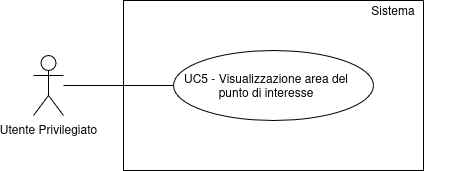
\includegraphics[width=0.7\linewidth]{UC5image.png}
    \caption{UC5 - Visualizzazione area del punto di interesse}
    \label{fig:UC5}
\end{figure}
\begin{itemize}
     \item \textbf{Attore$_G$ Principale:} Utente Privilegiato.
     \item \textbf{Precondizioni:}
        \begin{itemize}
    		\item L'utente privilegiato sta visualizzando la Dashboard$_G$ (UC1);
    	        \item L'utente privilegiato sta visualizzando i punti di interesse presenti sulla mappa (UC1.2);
    	        \item L'utente privilegiato ha selezionato un Marker$_G$, riferito ad un singolo punto di interesse (UC1.2.1).
            \item L'utente privilegiato ha selezionato un punto di interesse (UC1.2).
        \end{itemize}
     \item \textbf{Postcondizioni:} L'utente privilegiato è in grado di visualizzare l'area di influenza del punto di interesse selezionato sulla mappa.
     \item \textbf{Scenario Principale:}
        \begin{enumerate}
            \item Il Sistema$_G$ genera l'area di influenza del punto di interesse selezionato e la mostra sulla mappa.
        \end{enumerate}
     \item \textbf{User-Story$_G$ associata:}
     Come utente privilegiato voglio vedere l'area di influenza di ogni punto di interesse presente sulla mappa.
\end{itemize}

%%%%%%%%%%%%%%%%%%%%%%%%%%%%%%%%%%%%%%%%%%%%%%%%%%%%%%%%%%%%%%%%%%%%%%%%%%%
 \subsubsection{\textbf{UC6 - Visualizzazione informazioni del punto di interesse}}
\begin{figure}[H]
    \centering
    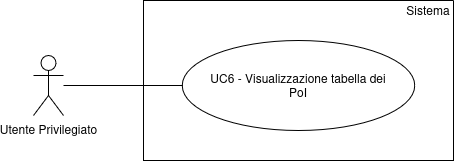
\includegraphics[width=0.7\linewidth]{UC6image.png}
    \caption{UC6 -- UC6.1 -- UC6.2 -- UC6.3 -- UC6.4 -- UC6.5 -- UC6.6}
    \label{fig:UC6}
\end{figure}
 \begin{itemize}
     \item \textbf{Attore$_G$ Principale:} Utente Privilegiato.
     \item \textbf{Precondizioni:}
       \begin{itemize}
    		\item L'utente privilegiato sta visualizzando la Dashboard$_G$ (UC1);
    	        \item L'utente privilegiato sta visualizzando i punti di interesse presenti sulla mappa (UC1.2/UC3.2);
    	        \item L'utente privilegiato ha selezionato un Marker$_G$, riferito ad un singolo punto di interesse (UC1.2.1/3.2.1).
       \end{itemize}
     \item \textbf{Postcondizioni:} L'utente privilegiato visualizza un pannello contenente una tabella, che esprime le informazioni specifiche del punto di interesse selezionato.
     \item \textbf{Scenario Principale:}
        \begin{enumerate}
          \item L'utente privilegiato ha selezionato un punto di interesse presente sulla mappa;
            \item Il Sistema$_G$ riporta le informazioni del punto di interesse selezionato e le mostra nella Dashboard$_G$ in forma tabellare. Tali informazioni sono:
       \begin{itemize}
       \item Il nome;
       \item La posizione espressa in latitudine e longitudine;
       \item L'indirizzo;
       \item La tipologia, cioè di che ambito si occupa il punto di interesse;
       \item La descrizione.
       \end{itemize}
        \end{enumerate}
     \item \textbf{User-Story$_G$ associata:} Come utente privilegiato voglio visualizzare le informazioni di un punto di interesse presente sulla mappa. 
 \end{itemize}
%%%%%%%%%%%%%%%%%%%%%%%%%%%%%%%%%%%%%%%%%%%%%%%%%%%%%%%%%%%%%%%%%%%%%%%%%%%
 \subsubsection{\textbf{UC6.1 - Visualizzazione latitudine del PoI}}
 \begin{itemize}
     \item \textbf{Attore$_G$ Principale:} Utente Privilegiato.
     \item \textbf{Precondizioni:}
       \begin{itemize}
    	        \item L'utente privilegiato ha selezionato un Marker$_G$, riferito ad un singolo punto di interesse (UC1.2.1/3.2.1);
          \item L'utente privilegiato sta visualizzando un pannello contenente la tabella delle informazioni del punto di interesse selezionato (UC6).
       \end{itemize}
     \item \textbf{Postcondizioni:} L'utente privilegiato visualizza la latitudine del punto di interesse selezionato.
     \item \textbf{Scenario Principale:}
        \begin{enumerate}
            \item L'utente privilegiato ha accesso alla Dashboard$_G$ (UC1);
            \item L'utente privilegiato seleziona un punto di interesse presente sulla mappa;
            \item Il Sistema$_G$ riporta le informazioni del punto di interesse in forma tabellare (UC6);
            \item La tabella conterrà la latitudine del punto di interesse selezionato.
        \end{enumerate}
     \item \textbf{User-Story$_G$ associata:} Come utente privilegiato voglio visualizzare la latitudine del punto di interesse selezionato. 
 \end{itemize}
%%%%%%%%%%%%%%%%%%%%%%%%%%%%%%%%%%%%%%%%%%%%%%%%%%%%%%%%%%%%%%%%%%%%%%%%%%%
 \subsubsection{\textbf{UC6.2 - Visualizzazione longitudine del PoI}}
 \begin{itemize}
     \item \textbf{Attore$_G$ Principale:} Utente Privilegiato.
     \item \textbf{Precondizioni:}
       \begin{itemize}
    	        \item L'utente privilegiato ha selezionato un Marker$_G$, riferito ad un singolo punto di interesse (UC1.2.1/3.2.1);
          \item L'utente privilegiato sta visualizzando un pannello contenente la tabella delle informazioni del punto di interesse selezionato (UC6).
       \end{itemize}
     \item \textbf{Postcondizioni:} L'utente privilegiato visualizza la longitudine del punto di interesse selezionato.
     \item \textbf{Scenario Principale:}
        \begin{enumerate}
            \item L'utente privilegiato ha accesso alla Dashboard$_G$ (UC1);
            \item L'utente privilegiato seleziona un punto di interesse presente sulla mappa;
            \item Il Sistema$_G$ riporta le informazioni del punto di interesse in forma tabellare (UC6);
            \item La tabella conterrà la longitudine del punto di interesse selezionato.
        \end{enumerate}
     \item \textbf{User-Story$_G$ associata:} Come utente privilegiato voglio visualizzare la longitudine del punto di interesse selezionato. 
 \end{itemize}
%%%%%%%%%%%%%%%%%%%%%%%%%%%%%%%%%%%%%%%%%%%%%%%%%%%%%%%%%%%%%%%%%%%%%%%%%%%
 \subsubsection{\textbf{UC6.3 - Visualizzazione nome del PoI}}
 \begin{itemize}
     \item \textbf{Attore$_G$ Principale:} Utente Privilegiato.
     \item \textbf{Precondizioni:}
       \begin{itemize}
    	        \item L'utente privilegiato ha selezionato un Marker$_G$, riferito ad un singolo punto di interesse (UC1.2.1/3.2.1);
          \item L'utente privilegiato sta visualizzando un pannello contenente la tabella delle informazioni del punto di interesse selezionato (UC6).
       \end{itemize}
     \item \textbf{Postcondizioni:} L'utente privilegiato visualizza il nome del punto di interesse selezionato.
     \item \textbf{Scenario Principale:}
        \begin{enumerate}
            \item L'utente privilegiato ha accesso alla Dashboard$_G$ (UC1);
            \item L'utente privilegiato seleziona un punto di interesse presente sulla mappa;
            \item Il Sistema$_G$ riporta le informazioni del punto di interesse in forma tabellare (UC6);
            \item La tabella conterrà il nome del punto di interesse selezionato.
        \end{enumerate}
     \item \textbf{User-Story$_G$ associata:} Come utente privilegiato voglio visualizzare il nome del punto di interesse selezionato. 
 \end{itemize}
%%%%%%%%%%%%%%%%%%%%%%%%%%%%%%%%%%%%%%%%%%%%%%%%%%%%%%%%%%%%%%%%%%%%%%%%%%%
 \subsubsection{\textbf{UC6.4 - Visualizzazione indirizzo del PoI}}
 \begin{itemize}
     \item \textbf{Attore$_G$ Principale:} Utente Privilegiato.
     \item \textbf{Precondizioni:}
       \begin{itemize}
    	        \item L'utente privilegiato ha selezionato un Marker$_G$, riferito ad un singolo punto di interesse (UC1.2.1/3.2.1);
          \item L'utente privilegiato sta visualizzando un pannello contenente la tabella delle informazioni del punto di interesse selezionato (UC6).
       \end{itemize}
     \item \textbf{Postcondizioni:} L'utente privilegiato visualizza l'indirizzo del punto di interesse selezionato.
     \item \textbf{Scenario Principale:}
        \begin{enumerate}
            \item L'utente privilegiato ha accesso alla Dashboard$_G$ (UC1);
            \item L'utente privilegiato seleziona un punto di interesse presente sulla mappa;
            \item Il Sistema$_G$ riporta le informazioni del punto di interesse in forma tabellare (UC6);
            \item La tabella conterrà l'indirizzo del punto di interesse selezionato.
        \end{enumerate}
     \item \textbf{User-Story$_G$ associata:} Come utente privilegiato voglio visualizzare l'indirizzo del punto di interesse selezionato. 
 \end{itemize}
%%%%%%%%%%%%%%%%%%%%%%%%%%%%%%%%%%%%%%%%%%%%%%%%%%%%%%%%%%%%%%%%%%%%%%%%%%%
 \subsubsection{\textbf{UC6.5 - Visualizzazione tipologia del PoI}}
 \begin{itemize}
     \item \textbf{Attore$_G$ Principale:} Utente Privilegiato.
     \item \textbf{Precondizioni:}
       \begin{itemize}
    	        \item L'utente privilegiato ha selezionato un Marker$_G$, riferito ad un singolo punto di interesse (UC1.2.1/3.2.1);
          \item L'utente privilegiato sta visualizzando un pannello contenente la tabella delle informazioni del punto di interesse selezionato (UC6).
       \end{itemize}
     \item \textbf{Postcondizioni:} L'utente privilegiato visualizza la tipologia del punto di interesse selezionato.
     \item \textbf{Scenario Principale:}
        \begin{enumerate}
            \item L'utente privilegiato ha accesso alla Dashboard$_G$ (UC1);
            \item L'utente privilegiato seleziona un punto di interesse presente sulla mappa;
            \item Il Sistema$_G$ riporta le informazioni del punto di interesse in forma tabellare (UC6);
            \item La tabella conterrà la tipologia del punto di interesse selezionato.
        \end{enumerate}
     \item \textbf{User-Story$_G$ associata:} Come utente privilegiato voglio visualizzare la tipologia del punto di interesse selezionato. 
 \end{itemize}
%%%%%%%%%%%%%%%%%%%%%%%%%%%%%%%%%%%%%%%%%%%%%%%%%%%%%%%%%%%%%%%%%%%%%%%%%%%
 \subsubsection{\textbf{UC6.6 - Visualizzazione descrizione del PoI}}
 \begin{itemize}
     \item \textbf{Attore$_G$ Principale:} Utente Privilegiato.
     \item \textbf{Precondizioni:}
       \begin{itemize}
    	        \item L'utente privilegiato ha selezionato un Marker$_G$, riferito ad un singolo punto di interesse (UC1.2.1/3.2.1);
          \item L'utente privilegiato sta visualizzando un pannello contenente la tabella delle informazioni del punto di interesse selezionato (UC6).
       \end{itemize}
     \item \textbf{Postcondizioni:} L'utente privilegiato visualizza la descrizione del punto di interesse selezionato.
     \item \textbf{Scenario Principale:}
        \begin{enumerate}
            \item L'utente privilegiato ha accesso alla Dashboard$_G$ (UC1);
            \item L'utente privilegiato seleziona un punto di interesse presente sulla mappa;
            \item Il Sistema$_G$ riporta le informazioni del punto di interesse in forma tabellare (UC6);
            \item La tabella conterrà la descrizione del punto di interesse selezionato.
        \end{enumerate}
     \item \textbf{User-Story$_G$ associata:} Come utente privilegiato voglio visualizzare la descrizione del punto di interesse selezionato. 
 \end{itemize}

%%%%%%%%%%%%%%%%%%%%%%%%%%%%%%%%%%%%%%%%%%%%%%%%%%%%%%%%%%%%%%%%%%%%%%%%%%%

%%%%%%%%%%%%%%%%%%%%%%%%%%%%%%%%%%%%%%%%%%%%%%%%%%%%%%%%%%%%%%%%%%%%%%%%%%%
\subsubsection{\textbf{UC7 - Visualizzazione tabella dei PoI}}
\begin{figure}[H]
    \centering
    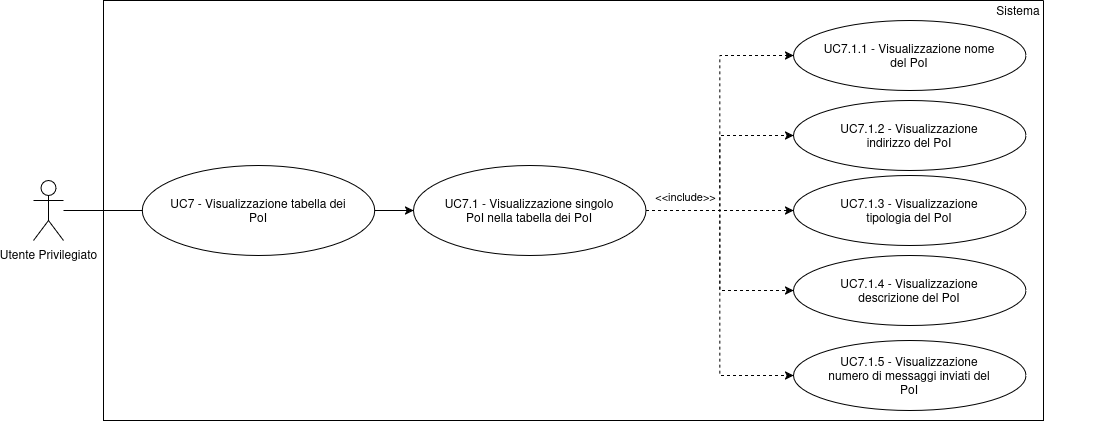
\includegraphics[width=0.7\linewidth]{UC7image.png}
    \caption{UC7 - Visualizzazione tabella dei PoI}
    \label{fig:UC7}
\end{figure}
\label{UC7}
\begin{itemize}
    \item \textbf{Attore$_G$ Principale:} Utente Privilegiato.
    \item \textbf{Precondizioni:} 
        \begin{itemize}
          \item Il Sistema$_G$ è operativo e accessibile.
        \end{itemize}
      \item \textbf{Postcondizioni:} L'utente privilegiato è in grado di visualizzare una tabella contenenti i dati dei singoli PoI ordinati per la quantità di messaggi inviati in questo mese.\\
    \item \textbf{Scenario Principale:} 
        \begin{enumerate}
        \item L'utente privilegiato seleziona la visualizzazione della tabella dei PoI;
          \item Il Sistema$_G$ mette a disposizioni le informazioni storicizzate per ogni singolo PoI in forma tabellare.
        \end{enumerate}
    \item \textbf{User-Story$_G$ associata:} Come utente privilegiato, voglio accedere alla tabella dei PoI per poter visualizzare quale PoI sta inviando più messaggi in quel mese e poter visionare facilmente le informazioni di ogni singolo PoI.
\end{itemize}

%%%%%%%%%%%%%%%%%%%%%%%%%%%%%%%%%%%%%%%%%%%%%%%%%%%%%%%%%%%%%%%%%%%%%%%%%%%
\subsubsection{\textbf{UC7.1 - Visualizzazione singolo PoI nella tabella dei PoI}}
\label{UC7.1}
\begin{itemize}
    \item \textbf{Attore$_G$ Principale:} Utente Privilegiato.
    \item \textbf{Precondizioni:} 
        \begin{itemize}
          \item Il Sistema$_G$ è operativo e accessibile;
            \item L'utente privilegiato sta visualizzando la tabella dei PoI (UC5).
        \end{itemize}
      \item \textbf{Postcondizioni:} L'utente privilegiato è in grado di visualizzare le informazioni di un singolo PoI.
    \item \textbf{Scenario Principale:} 
        \begin{enumerate}
        \item L'utente privilegiato seleziona la visualizzazione della tabella dei PoI;
          \item Il Sistema$_G$ mette a disposizioni le informazioni storicizzate per ogni singolo PoI in forma tabellare (UC5);
          \item L'utente privilegiato visualizza le informazioni di un singolo PoI nella tabella. Tali informazioni sono:
        \begin{itemize}
       \item Il nome;
       \item L'indirizzo;
       \item La tipologia, cioè di che ambito si occupa il punto di interesse;
       \item La descrizione;
         \item Numero di messaggi inviati durante il mese.
        \end{itemize}
        \end{enumerate}
    \item \textbf{User-Story$_G$ associata:} Come utente privilegiato, voglio poter visualizzare le informazioni di un singolo PoI.
\end{itemize}

%%%%%%%%%%%%%%%%%%%%%%%%%%%%%%%%%%%%%%%%%%%%%%%%%%%%%%%%%%%%%%%%%%%%%%%%%%%
\subsubsection{\textbf{UC7.1.1 - Visualizzazione nome del PoI}}
\label{UC7.1.1}
\begin{itemize}
    \item \textbf{Attore$_G$ Principale:} Utente Privilegiato.
    \item \textbf{Precondizioni:} 
        \begin{itemize}
          \item L'utente privilegiato sta visualizzando la tabella dei PoI (UC5);
            \item L'utente privilegiato sta visualizzando un singolo PoI nella tabella (UC5.1).
        \end{itemize}
      \item \textbf{Postcondizioni:} L'utente privilegiato è in grado di visualizzare il nome del singolo PoI.
    \item \textbf{Scenario Principale:} 
        \begin{enumerate}
        \item L'utente privilegiato seleziona la visualizzazione della tabella dei PoI;
          \item Il Sistema$_G$ mette a disposizioni le informazioni storicizzate per ogni singolo PoI in forma tabellare (UC5);
          \item L'utente privilegiato visualizza le informazioni di un singolo PoI nella tabella;
            \item L'utente privilegiato è in grado di visualizzare il nome di un singolo PoI.
        \end{enumerate}
    \item \textbf{User-Story$_G$ associata:} Come utente privilegiato, voglio poter visualizzare il nome di un singolo PoI.
\end{itemize}

%%%%%%%%%%%%%%%%%%%%%%%%%%%%%%%%%%%%%%%%%%%%%%%%%%%%%%%%%%%%%%%%%%%%%%%%%%%
\subsubsection{\textbf{UC7.1.2 - Visualizzazione indirizzo del PoI}}
\label{UC7.1.2}
\begin{itemize}
    \item \textbf{Attore$_G$ Principale:} Utente Privilegiato.
    \item \textbf{Precondizioni:} 
        \begin{itemize}
          \item L'utente privilegiato sta visualizzando la tabella dei PoI (UC5);
            \item L'utente privilegiato sta visualizzando un singolo PoI nella tabella (UC5.1).
        \end{itemize}
      \item \textbf{Postcondizioni:} L'utente privilegiato è in grado di visualizzare l'indirizzo del singolo PoI.
    \item \textbf{Scenario Principale:} 
        \begin{enumerate}
        \item L'utente privilegiato seleziona la visualizzazione della tabella dei PoI;
          \item Il Sistema$_G$ mette a disposizioni le informazioni storicizzate per ogni singolo PoI in forma tabellare (UC5);
          \item L'utente privilegiato visualizza le informazioni di un singolo PoI nella tabella;
            \item L'utente privilegiato è in grado di visualizzare l'indirizzo di un singolo PoI.
        \end{enumerate}
    \item \textbf{User-Story$_G$ associata:} Come utente privilegiato, voglio poter visualizzare l'indirizzo di un singolo PoI.
\end{itemize}
%%%%%%%%%%%%%%%%%%%%%%%%%%%%%%%%%%%%%%%%%%%%%%%%%%%%%%%%%%%%%%%%%%%%%%%%%%%
\subsubsection{\textbf{UC7.1.3 - Visualizzazione tipologia del PoI}}
\label{UC7.1.3}
\begin{itemize}
    \item \textbf{Attore$_G$ Principale:} Utente Privilegiato.
    \item \textbf{Precondizioni:} 
        \begin{itemize}
          \item L'utente privilegiato sta visualizzando la tabella dei PoI (UC5);
            \item L'utente privilegiato sta visualizzando un singolo PoI nella tabella (UC5.1).
        \end{itemize}
      \item \textbf{Postcondizioni:} L'utente privilegiato è in grado di visualizzare la tipologia del singolo PoI.
    \item \textbf{Scenario Principale:} 
        \begin{enumerate}
        \item L'utente privilegiato seleziona la visualizzazione della tabella dei PoI;
          \item Il Sistema$_G$ mette a disposizioni le informazioni storicizzate per ogni singolo PoI in forma tabellare (UC5);
          \item L'utente privilegiato visualizza le informazioni di un singolo PoI nella tabella;
            \item L'utente privilegiato è in grado di visualizzare la tipologia di un singolo PoI.
        \end{enumerate}
    \item \textbf{User-Story$_G$ associata:} Come utente privilegiato, voglio poter visualizzare la tipologia di un singolo PoI.
\end{itemize}
%%%%%%%%%%%%%%%%%%%%%%%%%%%%%%%%%%%%%%%%%%%%%%%%%%%%%%%%%%%%%%%%%%%%%%%%%%%
\subsubsection{\textbf{UC7.1.4 - Visualizzazione descrizione del PoI}}
\label{UC7.1.4}
\begin{itemize}
    \item \textbf{Attore$_G$ Principale:} Utente Privilegiato.
    \item \textbf{Precondizioni:} 
        \begin{itemize}
          \item L'utente privilegiato sta visualizzando la tabella dei PoI (UC5);
            \item L'utente privilegiato sta visualizzando un singolo PoI nella tabella (UC5.1).
        \end{itemize}
      \item \textbf{Postcondizioni:} L'utente privilegiato è in grado di visualizzare la descrizione del singolo PoI.
    \item \textbf{Scenario Principale:} 
        \begin{enumerate}
        \item L'utente privilegiato seleziona la visualizzazione della tabella dei PoI;
          \item Il Sistema$_G$ mette a disposizioni le informazioni storicizzate per ogni singolo PoI in forma tabellare (UC5);
          \item L'utente privilegiato visualizza le informazioni di un singolo PoI nella tabella;
            \item L'utente privilegiato è in grado di visualizzare la descrizione di un singolo PoI.
        \end{enumerate}
    \item \textbf{User-Story$_G$ associata:} Come utente privilegiato, voglio poter visualizzare la descrizione di un singolo PoI.
\end{itemize}
%%%%%%%%%%%%%%%%%%%%%%%%%%%%%%%%%%%%%%%%%%%%%%%%%%%%%%%%%%%%%%%%%%%%%%%%%%%
\subsubsection{\textbf{UC7.1.5 - Visualizzazione numero di messaggi inviati del PoI}}
\label{UC7.1.5}
\begin{itemize}
    \item \textbf{Attore$_G$ Principale:} Utente Privilegiato.
    \item \textbf{Precondizioni:} 
        \begin{itemize}
          \item L'utente privilegiato sta visualizzando la tabella dei PoI (UC5);
            \item L'utente privilegiato sta visualizzando un singolo PoI nella tabella (UC5.1).
        \end{itemize}
      \item \textbf{Postcondizioni:} L'utente privilegiato è in grado di visualizzare il numero di messaggi inviati dal singolo PoI durante il mese.
    \item \textbf{Scenario Principale:} 
        \begin{enumerate}
        \item L'utente privilegiato seleziona la visualizzazione della tabella dei PoI;
          \item Il Sistema$_G$ mette a disposizioni le informazioni storicizzate per ogni singolo PoI in forma tabellare (UC5);
          \item L'utente privilegiato visualizza le informazioni di un singolo PoI nella tabella;
            \item L'utente privilegiato è in grado di visualizzare il numero di messaggi inviati da un singolo PoI durante il mese.
        \end{enumerate}
    \item \textbf{User-Story$_G$ associata:} Come utente privilegiato, voglio poter visualizzare il numero di messaggi inviati da un singolo PoI.
\end{itemize}
%%%%%%%%%%%%%%%%%%%%%%%%%%%%%%%%%%%%%%%%%%%%%%%%%%%%%%%%%%%%%%%%%%%%%%%%%%%

\subsubsection{\textbf{UC8 - Visualizzazione informazioni dell'annuncio}}
\begin{figure}[H]
    \centering
    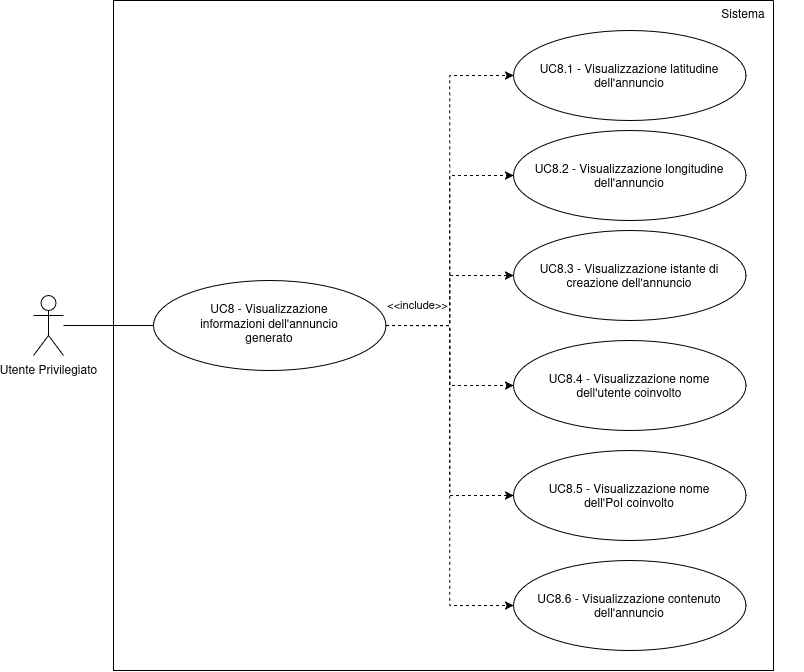
\includegraphics[width=0.7\linewidth]{UC8image.png}
    \caption{UC8 -- UC8.1 -- UC8.2 -- UC8.3 -- UC8.4 -- UC8.5 -- UC8.6}
    \label{fig:UC8}
\end{figure}
\label{UC8}
\begin{itemize}
    \item \textbf{Attore$_G$ Principale:} Utente privilegiato.
    \item \textbf{Precondizioni:} 
        \begin{itemize}
    	        \item L'utente privilegiato sta visualizzando gli annunci presenti sulla mappa (UC1.3/UC3.3);
    	        \item L'utente privilegiato ha selezionato un Marker$_G$, riferito ad un singolo annuncio (UC1.3.1/3.3.1).
        \end{itemize}
    \item \textbf{Postcondizioni:} L'utente privilegiato visualizza un pannello contenente le informazioni dell'annuncio selezionato in forma tabellare. 
    \item \textbf{Scenario Principale:} 
        \begin{enumerate}
          \item L'utente privilegiato ha selezionato un annuncio presente sulla mappa;
          \item Il Sistema$_G$ riporta le informazioni dell'annuncio selezionato e le mostra nella Dashboard$_G$ in forma tabellare;
          \item La tabella conterrà i nomi dell'utente e del punto di interesse coinvolti, la longitudine e latitudine di questi ultimi, il contenuto effettivo dell'annuncio e l'istante di creazione dell'annuncio.
	\end{enumerate}
    \item \textbf{User-Story$_G$ associata:} Come utente privilegiato voglio visualizzare le informazioni relative ad un annuncio pubblicitario.
\end{itemize}
%%%%%%%%%%%%%%%%%%%%%%%%%%%%%%%%%%%%%%%%%%%%%%%%%%%%%%%%%%%%%%%%%%%%%%%%%%%
 \subsubsection{\textbf{UC8.1 - Visualizzazione latitudine dell'annuncio}}
 \begin{itemize}
     \item \textbf{Attore$_G$ Principale:} Utente Privilegiato.
     \item \textbf{Precondizioni:}
       \begin{itemize}
    	        \item L'utente privilegiato ha selezionato un Marker$_G$, riferito ad un singolo annuncio (UC1.3.1/3.3.1).
          \item L'utente privilegiato sta visualizzando un pannello contenente la tabella delle informazioni dell'annuncio selezionato (UC8).
       \end{itemize}
     \item \textbf{Postcondizioni:} L'utente privilegiato visualizza la latitudine dell'annuncio selezionato.
     \item \textbf{Scenario Principale:}
        \begin{enumerate}
            \item L'utente privilegiato ha accesso alla Dashboard$_G$ (UC1);
            \item L'utente privilegiato seleziona un annuncio presente sulla mappa;
            \item Il Sistema$_G$ riporta le informazioni dell'annuncio in forma tabellare (UC8);
            \item La tabella conterrà la latitudine dell'annuncio selezionato.
        \end{enumerate}
     \item \textbf{User-Story$_G$ associata:} Come utente privilegiato voglio visualizzare la latitudine dell'annuncio selezionato. 
 \end{itemize}
%%%%%%%%%%%%%%%%%%%%%%%%%%%%%%%%%%%%%%%%%%%%%%%%%%%%%%%%%%%%%%%%%%%%%%%%%%%
 \subsubsection{\textbf{UC8.2 - Visualizzazione longitudine dell'annuncio}}
 \begin{itemize}
     \item \textbf{Attore$_G$ Principale:} Utente Privilegiato.
     \item \textbf{Precondizioni:}
       \begin{itemize}
    	        \item L'utente privilegiato ha selezionato un Marker$_G$, riferito ad un singolo annuncio (UC1.3.1/3.3.1).
          \item L'utente privilegiato sta visualizzando un pannello contenente la tabella delle informazioni dell'annuncio selezionato (UC8).
       \end{itemize}
     \item \textbf{Postcondizioni:} L'utente privilegiato visualizza la longitudine dell'annuncio selezionato.
     \item \textbf{Scenario Principale:}
        \begin{enumerate}
            \item L'utente privilegiato ha accesso alla Dashboard$_G$ (UC1);
            \item L'utente privilegiato seleziona un annuncio presente sulla mappa;
            \item Il Sistema$_G$ riporta le informazioni dell'annuncio in forma tabellare (UC8);
            \item La tabella conterrà la longitudine dell'annuncio selezionato.
        \end{enumerate}
     \item \textbf{User-Story$_G$ associata:} Come utente privilegiato voglio visualizzare la longitudine dell'annuncio selezionato. 
 \end{itemize}
%%%%%%%%%%%%%%%%%%%%%%%%%%%%%%%%%%%%%%%%%%%%%%%%%%%%%%%%%%%%%%%%%%%%%%%%%%%
 \subsubsection{\textbf{UC8.3 - Visualizzazione istante di creazione dell'annuncio}}
 \begin{itemize}
     \item \textbf{Attore$_G$ Principale:} Utente Privilegiato.
     \item \textbf{Precondizioni:}
       \begin{itemize}
    	        \item L'utente privilegiato ha selezionato un Marker$_G$, riferito ad un singolo annuncio (UC1.3.1/3.3.1).
          \item L'utente privilegiato sta visualizzando un pannello contenente la tabella delle informazioni dell'annuncio selezionato (UC8).
       \end{itemize}
     \item \textbf{Postcondizioni:} L'utente privilegiato visualizza l'istante di creazione dell'annuncio selezionato.
     \item \textbf{Scenario Principale:}
        \begin{enumerate}
            \item L'utente privilegiato ha accesso alla Dashboard$_G$ (UC1);
            \item L'utente privilegiato seleziona un annuncio presente sulla mappa;
            \item Il Sistema$_G$ riporta le informazioni dell'annuncio in forma tabellare (UC8);
            \item La tabella conterrà l'istante di creazione dell'annuncio selezionato.
        \end{enumerate}
     \item \textbf{User-Story$_G$ associata:} Come utente privilegiato voglio visualizzare l'istante di creazione dell'annuncio selezionato. 
 \end{itemize}
%%%%%%%%%%%%%%%%%%%%%%%%%%%%%%%%%%%%%%%%%%%%%%%%%%%%%%%%%%%%%%%%%%%%%%%%%%%
 \subsubsection{\textbf{UC8.4 - Visualizzazione nome dell'utente coinvolto}}
 \begin{itemize}
     \item \textbf{Attore$_G$ Principale:} Utente Privilegiato.
     \item \textbf{Precondizioni:}
       \begin{itemize}
    	        \item L'utente privilegiato ha selezionato un Marker$_G$, riferito ad un singolo annuncio (UC1.3.1/3.3.1).
          \item L'utente privilegiato sta visualizzando un pannello contenente la tabella delle informazioni dell'annuncio selezionato (UC8).
       \end{itemize}
     \item \textbf{Postcondizioni:} L'utente privilegiato visualizza il nome dell'utente a cui l'annuncio selezionato è riferito.
     \item \textbf{Scenario Principale:}
        \begin{enumerate}
            \item L'utente privilegiato ha accesso alla Dashboard$_G$ (UC1);
            \item L'utente privilegiato seleziona un annuncio presente sulla mappa;
            \item Il Sistema$_G$ riporta le informazioni dell'annuncio in forma tabellare (UC8);
            \item La tabella conterrà il nome dell'utente a cui l'annuncio selezionato è riferito.
        \end{enumerate}
     \item \textbf{User-Story$_G$ associata:} Come utente privilegiato voglio visualizzare il nome dell'utente a cui l'annuncio selezionato è riferito. 
 \end{itemize}
%%%%%%%%%%%%%%%%%%%%%%%%%%%%%%%%%%%%%%%%%%%%%%%%%%%%%%%%%%%%%%%%%%%%%%%%%%%
 \subsubsection{\textbf{UC8.5 - Visualizzazione nome del PoI coinvolto}}
 \begin{itemize}
     \item \textbf{Attore$_G$ Principale:} Utente Privilegiato.
     \item \textbf{Precondizioni:}
       \begin{itemize}
    	        \item L'utente privilegiato ha selezionato un Marker$_G$, riferito ad un singolo annuncio (UC1.3.1/3.3.1).
          \item L'utente privilegiato sta visualizzando un pannello contenente la tabella delle informazioni dell'annuncio selezionato (UC8).
       \end{itemize}
     \item \textbf{Postcondizioni:} L'utente privilegiato visualizza il nome del PoI a cui l'annuncio selezionato è riferito.
     \item \textbf{Scenario Principale:}
        \begin{enumerate}
            \item L'utente privilegiato ha accesso alla Dashboard$_G$ (UC1);
            \item L'utente privilegiato seleziona un annuncio presente sulla mappa;
            \item Il Sistema$_G$ riporta le informazioni dell'annuncio in forma tabellare (UC8);
            \item La tabella conterrà il nome del PoI a cui l'annuncio selezionato è riferito.
        \end{enumerate}
     \item \textbf{User-Story$_G$ associata:} Come utente privilegiato voglio visualizzare il nome del PoI a cui l'annuncio selezionato è riferito. 
 \end{itemize}
%%%%%%%%%%%%%%%%%%%%%%%%%%%%%%%%%%%%%%%%%%%%%%%%%%%%%%%%%%%%%%%%%%%%%%%%%%%
 \subsubsection{\textbf{UC8.6 - Visualizzazione contenuto dell'annuncio}}
 \begin{itemize}
     \item \textbf{Attore$_G$ Principale:} Utente Privilegiato.
     \item \textbf{Precondizioni:}
       \begin{itemize}
    	        \item L'utente privilegiato ha selezionato un Marker$_G$, riferito ad un singolo annuncio (UC1.3.1/3.3.1).
          \item L'utente privilegiato sta visualizzando un pannello contenente la tabella delle informazioni dell'annuncio selezionato (UC8).
       \end{itemize}
     \item \textbf{Postcondizioni:} L'utente privilegiato visualizza il contenuto dell'annuncio selezionato.
     \item \textbf{Scenario Principale:}
        \begin{enumerate}
            \item L'utente privilegiato ha accesso alla Dashboard$_G$ (UC1);
            \item L'utente privilegiato seleziona un annuncio presente sulla mappa;
            \item Il Sistema$_G$ riporta le informazioni dell'annuncio in forma tabellare (UC8);
            \item La tabella conterrà il contenuto dell'annuncio selezionato.
        \end{enumerate}
     \item \textbf{User-Story$_G$ associata:} Come utente privilegiato voglio visualizzare il contenuto dell'annuncio selezionato. 
 \end{itemize}
%%%%%%%%%%%%%%%%%%%%%%%%%%%%%%%%%%%%%%%%%%%%%%%%%%%%%%%%%%%%%%%%%%%%%%%%%%%
\subsubsection{\textbf{UC9 - Trasmissione dati geoposizionali}}
\begin{figure}[H]
    \centering
    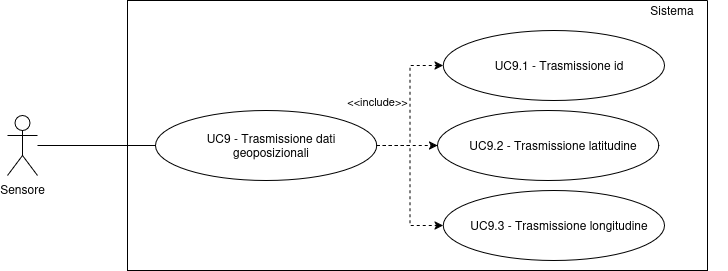
\includegraphics[width=0.7\linewidth]{UC9image.png}
    \caption{UC9 -- UC9.1 -- UC9.2 -- UC9.3}
    \label{fig:UC9}
\end{figure}
\label{UC9}
\begin{itemize}
    \item \textbf{Attore$_G$ Principale:} Sensore.
    \item \textbf{Precondizioni:} 
        \begin{itemize}
    	\item Il sensore è attivo e connesso al Sistema$_G$.
        \end{itemize}
    \item \textbf{Postcondizioni:} Il sensore invia i dati posizionali del mezzo al Sistema$_G$. Il Sistema$_G$ salva i dati inviati dal sensore. 
    \item \textbf{Scenario Principale:} 
        \begin{enumerate}
            \item Il sensore di tipo GPS effettua un rilevamento della posizione geografica dell'utente espressa in latitudine e longitudine;
            \item Il sensore GPS invia i dati posizionali al Sistema$_G$.
        \end{enumerate}
    \item \textbf{User-Story$_G$ associata:} Come Sensore GPS, desidero trasmettere la posizione espressa in latitudine e longitudine al Sistema$_G$.
\end{itemize}
%%%%%%%%%%%%%%%%%%%%%%%%%%%%%%%%%%%%%%%%%%%%%%%%%%%%%%%%%%%%%%%%%%%%%%%%%%%
\subsubsection{\textbf{UC9.1 - Trasmissione id}}
\begin{itemize}
    \item \textbf{Attore$_G$ Principale:} Sensore.
    \item \textbf{Precondizioni:} 
        \begin{itemize}
    	\item Il sensore è attivo e connesso al Sistema$_G$;
          \item Il sensore ha trasmesso i dati al Sistema$_G$.
        \end{itemize}
    \item \textbf{Postcondizioni:} Il sensore invia il suo id al Sistema$_G$.
    \item \textbf{Scenario Principale:} 
        \begin{enumerate}
            \item Il sensore di tipo GPS effettua un rilevamento della posizione geografica dell'utente espressa in latitudine e longitudine;
            \item Il sensore GPS invia i dati posizionali al Sistema$_G$;
            \item Il sensore GPS invia il proprio id.
        \end{enumerate}
    \item \textbf{User-Story$_G$ associata:} Come Sensore GPS, desidero trasmettere il mio id al Sistema$_G$.
\end{itemize}
%%%%%%%%%%%%%%%%%%%%%%%%%%%%%%%%%%%%%%%%%%%%%%%%%%%%%%%%%%%%%%%%%%%%%%%%%%%
\subsubsection{\textbf{UC9.2 - Trasmissione latitudine}}
\begin{itemize}
    \item \textbf{Attore$_G$ Principale:} Sensore.
    \item \textbf{Precondizioni:} 
        \begin{itemize}
    	\item Il sensore è attivo e connesso al Sistema$_G$;
          \item Il sensore ha trasmesso i dati al Sistema$_G$.
        \end{itemize}
    \item \textbf{Postcondizioni:} Il sensore invia la sua latitudine al Sistema$_G$.
    \item \textbf{Scenario Principale:} 
        \begin{enumerate}
            \item Il sensore di tipo GPS effettua un rilevamento della posizione geografica dell'utente espressa in latitudine e longitudine;
            \item Il sensore GPS invia i dati posizionali al Sistema$_G$;
            \item Il sensore GPS invia la sua latitudine.
        \end{enumerate}
    \item \textbf{User-Story$_G$ associata:} Come Sensore GPS, desidero trasmettere la mia latitudine al Sistema$_G$.
\end{itemize}
%%%%%%%%%%%%%%%%%%%%%%%%%%%%%%%%%%%%%%%%%%%%%%%%%%%%%%%%%%%%%%%%%%%%%%%%%%%
\subsubsection{\textbf{UC9.3 - Trasmissione longitudine}}
\begin{itemize}
    \item \textbf{Attore$_G$ Principale:} Sensore.
    \item \textbf{Precondizioni:} 
        \begin{itemize}
    	\item Il sensore è attivo e connesso al Sistema$_G$;
          \item Il sensore ha trasmesso i dati al Sistema$_G$.
        \end{itemize}
    \item \textbf{Postcondizioni:} Il sensore invia la sua longitudine al Sistema$_G$.
    \item \textbf{Scenario Principale:} 
        \begin{enumerate}
            \item Il sensore di tipo GPS effettua un rilevamento della posizione geografica dell'utente espressa in latitudine e longitudine;
            \item Il sensore GPS invia i dati posizionali al Sistema$_G$;
            \item Il sensore GPS invia la sua longitudine.
        \end{enumerate}
    \item \textbf{User-Story$_G$ associata:} Come Sensore GPS, desidero trasmettere la mia longitudine al Sistema$_G$.
\end{itemize}

%%%%%%%%%%%%%%%%%%%%%%%%%%%%%%%%%%%%%%%%%%%%%%%%%%%%%%%%%%%%%%%%%%%%%%%%%%%

\subsubsection{\textbf{UC10 - Ricezione dati utente e PoI}}
\begin{figure}[H]
    \centering
    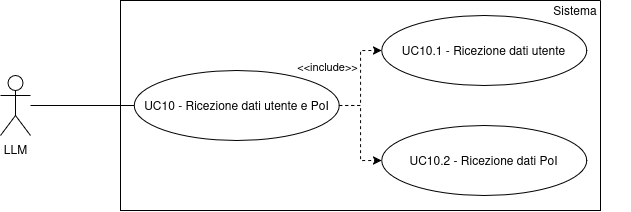
\includegraphics[width=0.7\linewidth]{UC10image.png}
    \caption{UC10 - Ricezione dati utente e PoI -- UC10.1 - Ricezione dati utente -- UC10.2 - Ricezione dati PoI}
    \label{fig:UC10}
\end{figure}
\label{UC10}
\begin{itemize}
    \item \textbf{Attore$_G$ Principale:} LLM$_G$.
    \item \textbf{Precondizioni:} 
        \begin{itemize}
        \item Il Sistema$_G$ è operativo e accessibile;
          \item Il Sistema$_G$ invia i dati dell'utente e del PoI selezionati all'LLM.
        \end{itemize}
      \item \textbf{Postcondizioni:} L'LLM riceve i dati dell'utente e del PoI selezionati dal Sistema$_G$.
    \item \textbf{Scenario Principale:} 
        \begin{enumerate}
          \item Il Sistema$_G$ invia i dati dell'utente e del PoI all'LLM;
        \item L' LLM$_G$ riceve i dati personali dell'utente e quelli del punto di interesse presente nelle vicinanze dell'utente.
        \end{enumerate}
      \item \textbf{User-Story$_G$ associata:} Come LLM$_G$ voglio ricevere i dati dell'utente e del PoI selezionati dal Sistema$_G$.
        identificare e selezionare il Punto di Interesse più rilevante per l'utente in base alla sua profilazione e alle sue preferenze.
\end{itemize}
%%%%%%%%%%%%%%%%%%%%%%%%%%%%%%%%%%%%%%%%%%%%%%%%%%%%%%%%%%%%%%%%%%%%%%%%%%%
\subsubsection{\textbf{UC10.1 - Ricezione dati utente}}
\begin{figure}[H]
    \centering
    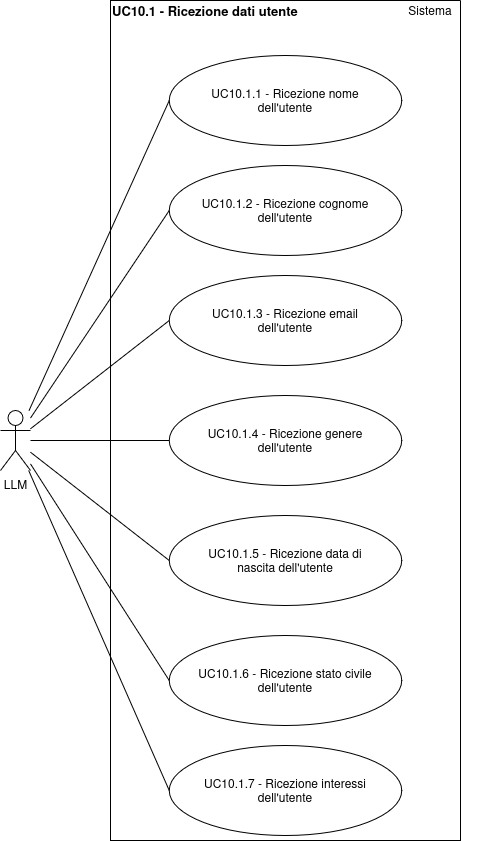
\includegraphics[width=0.7\linewidth]{UC10.1image.png}
    \caption{UC10.1.1 -- UC10.1.2 -- UC10.1.3 -- UC10.1.4 -- UC10.1.5 -- UC10.1.6 -- UC10.1.7}
    \label{fig:UC10.1}
\end{figure}
\label{UC10.1}
\begin{itemize}
    \item \textbf{Attore$_G$ Principale:} LLM$_G$.
    \item \textbf{Precondizioni:} 
        \begin{itemize}
          \item Il Sistema$_G$ è operativo e accessibile;
          \item Il Sistema$_G$ invia i dati dell'utente e del PoI selezionati all'LLM;
            \item L'LLM riceve i dati dell'utente e del PoI selezionati dal Sistema$_G$.
        \end{itemize}
      \item \textbf{Postcondizioni:} L'LLM riceve i dati dell'utente selezionato dal Sistema$_G$.
    \item \textbf{Scenario Principale:} 
        \begin{enumerate}
          \item Il Sistema$_G$ invia i dati dell'utente e del PoI all'LLM;
        \item L' LLM$_G$ riceve i dati personali dell'utente e quelli del punto di interesse presente nelle vicinanze dell'utente;
          \item L'LLM riceve le informazioni personali dell'utente, quali:
          \begin{itemize}
          \item Nome;
          \item Cognome;
          \item Email;
          \item Genere;
          \item Data di nascita;
          \item Stato civile;
          \item Elenco di interessi dell'utente.
          \end{itemize}
        \end{enumerate}
      \item \textbf{User-Story$_G$ associata:} Come LLM$_G$ voglio ricevere i dati dell'utente selezionato dal Sistema$_G$.
\end{itemize}
%%%%%%%%%%%%%%%%%%%%%%%%%%%%%%%%%%%%%%%%%%%%%%%%%%%%%%%%%%%%%%%%%%%%%%%%%%%
\subsubsection{\textbf{UC10.1.1 - Ricezione nome dell'utente}}
\begin{itemize}
    \item \textbf{Attore$_G$ Principale:} LLM$_G$.
    \item \textbf{Precondizioni:} 
        \begin{itemize}
          \item Il Sistema$_G$ è operativo e accessibile;
          \item Il Sistema$_G$ invia i dati dell'utente e del PoI selezionati all'LLM;
            \item L'LLM riceve i dati dell'utente e del PoI selezionati dal Sistema$_G$.
        \end{itemize}
      \item \textbf{Postcondizioni:} L'LLM riceve il nome dell'utente selezionato dal Sistema$_G$.
    \item \textbf{Scenario Principale:} 
        \begin{enumerate}
          \item Il Sistema$_G$ invia i dati dell'utente e del PoI all'LLM;
        \item L' LLM$_G$ riceve i dati personali dell'utente e quelli del punto di interesse presente nelle vicinanze dell'utente;
          \item L'LLM riceve le informazioni personali dell'utente;
          \item L'LLM riceve il nome dell'utente.
        \end{enumerate}
      \item \textbf{User-Story$_G$ associata:} Come LLM$_G$ voglio ricevere il nome dell'utente selezionato dal Sistema$_G$.
\end{itemize}
%%%%%%%%%%%%%%%%%%%%%%%%%%%%%%%%%%%%%%%%%%%%%%%%%%%%%%%%%%%%%%%%%%%%%%%%%%%
\subsubsection{\textbf{UC10.1.2 - Ricezione cognome dell'utente}}
\begin{itemize}
    \item \textbf{Attore$_G$ Principale:} LLM$_G$.
    \item \textbf{Precondizioni:} 
        \begin{itemize}
          \item Il Sistema$_G$ è operativo e accessibile;
          \item Il Sistema$_G$ invia i dati dell'utente e del PoI selezionati all'LLM;
            \item L'LLM riceve i dati dell'utente e del PoI selezionati dal Sistema$_G$.
        \end{itemize}
      \item \textbf{Postcondizioni:} L'LLM riceve il cognome dell'utente selezionato dal Sistema$_G$.
    \item \textbf{Scenario Principale:} 
        \begin{enumerate}
          \item Il Sistema$_G$ invia i dati dell'utente e del PoI all'LLM;
        \item L' LLM$_G$ riceve i dati personali dell'utente e quelli del punto di interesse presente nelle vicinanze dell'utente;
          \item L'LLM riceve le informazioni personali dell'utente;
          \item L'LLM riceve il cognome dell'utente.
        \end{enumerate}
      \item \textbf{User-Story$_G$ associata:} Come LLM$_G$ voglio ricevere il cognome dell'utente selezionato dal Sistema$_G$.
\end{itemize}
%%%%%%%%%%%%%%%%%%%%%%%%%%%%%%%%%%%%%%%%%%%%%%%%%%%%%%%%%%%%%%%%%%%%%%%%%%%
\subsubsection{\textbf{UC10.1.3 - Ricezione email dell'utente}}
\begin{itemize}
    \item \textbf{Attore$_G$ Principale:} LLM$_G$.
    \item \textbf{Precondizioni:} 
        \begin{itemize}
          \item Il Sistema$_G$ è operativo e accessibile;
          \item Il Sistema$_G$ invia i dati dell'utente e del PoI selezionati all'LLM;
            \item L'LLM riceve i dati dell'utente e del PoI selezionati dal Sistema$_G$.
        \end{itemize}
      \item \textbf{Postcondizioni:} L'LLM riceve l'email dell'utente selezionato dal Sistema$_G$.
    \item \textbf{Scenario Principale:} 
        \begin{enumerate}
          \item Il Sistema$_G$ invia i dati dell'utente e del PoI all'LLM;
        \item L' LLM$_G$ riceve i dati personali dell'utente e quelli del punto di interesse presente nelle vicinanze dell'utente;
          \item L'LLM riceve le informazioni personali dell'utente;
          \item L'LLM riceve l'email dell'utente.
        \end{enumerate}
      \item \textbf{User-Story$_G$ associata:} Come LLM$_G$ voglio ricevere l'email dell'utente selezionato dal Sistema$_G$.
\end{itemize}
%%%%%%%%%%%%%%%%%%%%%%%%%%%%%%%%%%%%%%%%%%%%%%%%%%%%%%%%%%%%%%%%%%%%%%%%%%%
\subsubsection{\textbf{UC10.1.4 - Ricezione genere dell'utente}}
\begin{itemize}
    \item \textbf{Attore$_G$ Principale:} LLM$_G$.
    \item \textbf{Precondizioni:} 
        \begin{itemize}
          \item Il Sistema$_G$ è operativo e accessibile;
          \item Il Sistema$_G$ invia i dati dell'utente e del PoI selezionati all'LLM;
            \item L'LLM riceve i dati dell'utente e del PoI selezionati dal Sistema$_G$.
        \end{itemize}
      \item \textbf{Postcondizioni:} L'LLM riceve il genere dell'utente selezionato dal Sistema$_G$.
    \item \textbf{Scenario Principale:} 
        \begin{enumerate}
          \item Il Sistema$_G$ invia i dati dell'utente e del PoI all'LLM;
        \item L' LLM$_G$ riceve i dati personali dell'utente e quelli del punto di interesse presente nelle vicinanze dell'utente;
          \item L'LLM riceve le informazioni personali dell'utente;
          \item L'LLM riceve il genere dell'utente.
        \end{enumerate}
      \item \textbf{User-Story$_G$ associata:} Come LLM$_G$ voglio ricevere il genere dell'utente selezionato dal Sistema$_G$.
\end{itemize}
%%%%%%%%%%%%%%%%%%%%%%%%%%%%%%%%%%%%%%%%%%%%%%%%%%%%%%%%%%%%%%%%%%%%%%%%%%%
\subsubsection{\textbf{UC10.1.5 - Ricezione data di nascita dell'utente}}
\begin{itemize}
    \item \textbf{Attore$_G$ Principale:} LLM$_G$.
    \item \textbf{Precondizioni:} 
        \begin{itemize}
          \item Il Sistema$_G$ è operativo e accessibile;
          \item Il Sistema$_G$ invia i dati dell'utente e del PoI selezionati all'LLM;
            \item L'LLM riceve i dati dell'utente e del PoI selezionati dal Sistema$_G$.
        \end{itemize}
      \item \textbf{Postcondizioni:} L'LLM riceve la data di nascita dell'utente selezionato dal Sistema$_G$.
    \item \textbf{Scenario Principale:} 
        \begin{enumerate}
          \item Il Sistema$_G$ invia i dati dell'utente e del PoI all'LLM;
        \item L' LLM$_G$ riceve i dati personali dell'utente e quelli del punto di interesse presente nelle vicinanze dell'utente;
          \item L'LLM riceve le informazioni personali dell'utente;
          \item L'LLM riceve la data di nascita dell'utente.
        \end{enumerate}
      \item \textbf{User-Story$_G$ associata:} Come LLM$_G$ voglio ricevere la data di nascita dell'utente selezionato dal Sistema$_G$.
\end{itemize}
%%%%%%%%%%%%%%%%%%%%%%%%%%%%%%%%%%%%%%%%%%%%%%%%%%%%%%%%%%%%%%%%%%%%%%%%%%%
\subsubsection{\textbf{UC10.1.6 - Ricezione stato civile dell'utente}}
\begin{itemize}
    \item \textbf{Attore$_G$ Principale:} LLM$_G$.
    \item \textbf{Precondizioni:} 
        \begin{itemize}
          \item Il Sistema$_G$ è operativo e accessibile;
          \item Il Sistema$_G$ invia i dati dell'utente e del PoI selezionati all'LLM;
            \item L'LLM riceve i dati dell'utente e del PoI selezionati dal Sistema$_G$.
        \end{itemize}
      \item \textbf{Postcondizioni:} L'LLM riceve lo stato civile dell'utente selezionato dal Sistema$_G$.
    \item \textbf{Scenario Principale:} 
        \begin{enumerate}
          \item Il Sistema$_G$ invia i dati dell'utente e del PoI all'LLM;
        \item L' LLM$_G$ riceve i dati personali dell'utente e quelli del punto di interesse presente nelle vicinanze dell'utente;
          \item L'LLM riceve le informazioni personali dell'utente;
          \item L'LLM riceve lo stato civile dell'utente.
        \end{enumerate}
      \item \textbf{User-Story$_G$ associata:} Come LLM$_G$ voglio ricevere lo stato civile dell'utente selezionato dal Sistema$_G$.
\end{itemize}
%%%%%%%%%%%%%%%%%%%%%%%%%%%%%%%%%%%%%%%%%%%%%%%%%%%%%%%%%%%%%%%%%%%%%%%%%%%
\subsubsection{\textbf{UC10.1.7 - Ricezione interessi dell'utente}}
\begin{itemize}
    \item \textbf{Attore$_G$ Principale:} LLM$_G$.
    \item \textbf{Precondizioni:} 
        \begin{itemize}
          \item Il Sistema$_G$ è operativo e accessibile;
          \item Il Sistema$_G$ invia i dati dell'utente e del PoI selezionati all'LLM;
            \item L'LLM riceve i dati dell'utente e del PoI selezionati dal Sistema$_G$.
        \end{itemize}
      \item \textbf{Postcondizioni:} L'LLM riceve gli interessi dell'utente selezionato dal Sistema$_G$.
    \item \textbf{Scenario Principale:} 
        \begin{enumerate}
          \item Il Sistema$_G$ invia i dati dell'utente e del PoI all'LLM;
        \item L' LLM$_G$ riceve i dati personali dell'utente e quelli del punto di interesse presente nelle vicinanze dell'utente;
          \item L'LLM riceve le informazioni personali dell'utente;
          \item L'LLM riceve gli interessi dell'utente.
        \end{enumerate}
      \item \textbf{User-Story$_G$ associata:} Come LLM$_G$ voglio ricevere gli interessi dell'utente selezionato dal Sistema$_G$.
\end{itemize}
%%%%%%%%%%%%%%%%%%%%%%%%%%%%%%%%%%%%%%%%%%%%%%%%%%%%%%%%%%%%%%%%%%%%%%%%%%%
\subsubsection{\textbf{UC10.2 - Ricezione dati PoI}}
\begin{figure}[H]
    \centering
    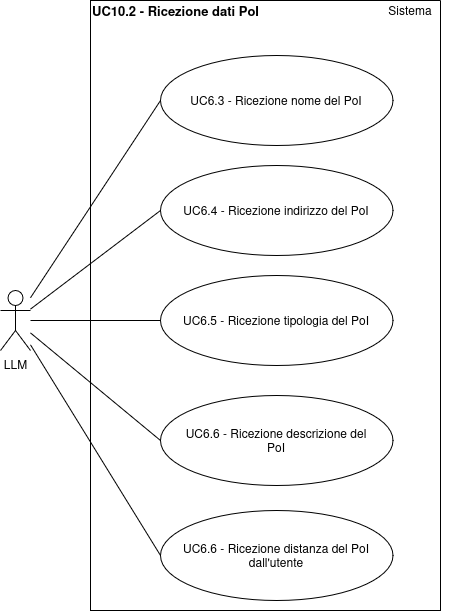
\includegraphics[width=0.7\linewidth]{UC10.2image.png}
    \caption{UC10.2.1 -- UC10.2.2 -- UC10.2.3 -- UC10.2.4 -- UC10.2.5}
    \label{fig:UC10.2}
\end{figure}
\label{UC10.2}
\begin{itemize}
    \item \textbf{Attore$_G$ Principale:} LLM$_G$.
    \item \textbf{Precondizioni:} 
        \begin{itemize}
          \item Il Sistema$_G$ è operativo e accessibile;
          \item Il Sistema$_G$ invia i dati dell'utente e del PoI selezionati all'LLM;
            \item L'LLM riceve i dati dell'utente e del PoI selezionati dal Sistema$_G$.
        \end{itemize}
      \item \textbf{Postcondizioni:} L'LLM riceve i dati del PoI selezionato dal Sistema$_G$.
    \item \textbf{Scenario Principale:} 
        \begin{enumerate}
          \item Il Sistema$_G$ invia i dati dell'utente e del PoI all'LLM;
          \item L' LLM$_G$ riceve i dati personali dell'utente e quelli del punto di interesse presente nelle vicinanze dell'utente;
          \item L'LLM riceve le informazioni del PoI, quali:
          \begin{itemize}
          \item Nome;
          \item Indirizzo;
          \item Tipologia, cioè di che ambito si occupa il punto di interesse;
          \item Descrizione;
          \item Distanza del PoI dall'utente.
          \end{itemize}
        \end{enumerate}
      \item \textbf{User-Story$_G$ associata:} Come LLM$_G$ voglio ricevere i dati del PoI selezionato dal Sistema$_G$.
\end{itemize}
%%%%%%%%%%%%%%%%%%%%%%%%%%%%%%%%%%%%%%%%%%%%%%%%%%%%%%%%%%%%%%%%%%%%%%%%%%%
\subsubsection{\textbf{UC10.2.1 - Ricezione nome del PoI}}
\begin{itemize}
    \item \textbf{Attore$_G$ Principale:} LLM$_G$.
    \item \textbf{Precondizioni:} 
        \begin{itemize}
          \item Il Sistema$_G$ è operativo e accessibile;
          \item Il Sistema$_G$ invia i dati dell'utente e del PoI selezionati all'LLM;
            \item L'LLM riceve i dati dell'utente e del PoI selezionati dal Sistema$_G$.
        \end{itemize}
      \item \textbf{Postcondizioni:} L'LLM riceve il nome del PoI selezionato dal Sistema$_G$.
    \item \textbf{Scenario Principale:} 
        \begin{enumerate}
          \item Il Sistema$_G$ invia i dati dell'utente e del PoI all'LLM;
        \item L' LLM$_G$ riceve i dati personali dell'utente e quelli del punto di interesse presente nelle vicinanze dell'utente;
          \item L'LLM riceve le informazioni del PoI;
          \item L'LLM riceve il nome del PoI.
        \end{enumerate}
      \item \textbf{User-Story$_G$ associata:} Come LLM$_G$ voglio ricevere il nome del PoI selezionato dal Sistema$_G$.
\end{itemize}
%%%%%%%%%%%%%%%%%%%%%%%%%%%%%%%%%%%%%%%%%%%%%%%%%%%%%%%%%%%%%%%%%%%%%%%%%%%
\subsubsection{\textbf{UC10.2.2 - Ricezione indirizzo del PoI}}
\begin{itemize}
    \item \textbf{Attore$_G$ Principale:} LLM$_G$.
    \item \textbf{Precondizioni:} 
        \begin{itemize}
          \item Il Sistema$_G$ è operativo e accessibile;
          \item Il Sistema$_G$ invia i dati dell'utente e del PoI selezionati all'LLM;
            \item L'LLM riceve i dati dell'utente e del PoI selezionati dal Sistema$_G$.
        \end{itemize}
      \item \textbf{Postcondizioni:} L'LLM riceve l'indirizzo del PoI selezionato dal Sistema$_G$.
    \item \textbf{Scenario Principale:} 
        \begin{enumerate}
          \item Il Sistema$_G$ invia i dati dell'utente e del PoI all'LLM;
        \item L' LLM$_G$ riceve i dati personali dell'utente e quelli del punto di interesse presente nelle vicinanze dell'utente;
          \item L'LLM riceve le informazioni del PoI;
          \item L'LLM riceve l'indirizzo del PoI.
        \end{enumerate}
      \item \textbf{User-Story$_G$ associata:} Come LLM$_G$ voglio ricevere l'indirizzo del PoI selezionato dal Sistema$_G$.
\end{itemize}
%%%%%%%%%%%%%%%%%%%%%%%%%%%%%%%%%%%%%%%%%%%%%%%%%%%%%%%%%%%%%%%%%%%%%%%%%%%
\subsubsection{\textbf{UC10.2.3 - Ricezione tipologia del PoI}}
\begin{itemize}
    \item \textbf{Attore$_G$ Principale:} LLM$_G$.
    \item \textbf{Precondizioni:} 
        \begin{itemize}
          \item Il Sistema$_G$ è operativo e accessibile;
          \item Il Sistema$_G$ invia i dati dell'utente e del PoI selezionati all'LLM;
            \item L'LLM riceve i dati dell'utente e del PoI selezionati dal Sistema$_G$.
        \end{itemize}
      \item \textbf{Postcondizioni:} L'LLM riceve la tipologia del PoI selezionato dal Sistema$_G$.
    \item \textbf{Scenario Principale:} 
        \begin{enumerate}
          \item Il Sistema$_G$ invia i dati dell'utente e del PoI all'LLM;
        \item L' LLM$_G$ riceve i dati personali dell'utente e quelli del punto di interesse presente nelle vicinanze dell'utente;
          \item L'LLM riceve le informazioni del PoI;
          \item L'LLM riceve la tipologia del PoI.
        \end{enumerate}
      \item \textbf{User-Story$_G$ associata:} Come LLM$_G$ voglio ricevere la tipologia del PoI selezionato dal Sistema$_G$.
\end{itemize}
%%%%%%%%%%%%%%%%%%%%%%%%%%%%%%%%%%%%%%%%%%%%%%%%%%%%%%%%%%%%%%%%%%%%%%%%%%%
\subsubsection{\textbf{UC10.2.4 - Ricezione descrizione del PoI}}
\begin{itemize}
    \item \textbf{Attore$_G$ Principale:} LLM$_G$.
    \item \textbf{Precondizioni:} 
        \begin{itemize}
          \item Il Sistema$_G$ è operativo e accessibile;
          \item Il Sistema$_G$ invia i dati dell'utente e del PoI selezionati all'LLM;
            \item L'LLM riceve i dati dell'utente e del PoI selezionati dal Sistema$_G$.
        \end{itemize}
      \item \textbf{Postcondizioni:} L'LLM riceve la descrizione del PoI selezionato dal Sistema$_G$.
    \item \textbf{Scenario Principale:} 
        \begin{enumerate}
          \item Il Sistema$_G$ invia i dati dell'utente e del PoI all'LLM;
        \item L' LLM$_G$ riceve i dati personali dell'utente e quelli del punto di interesse presente nelle vicinanze dell'utente;
          \item L'LLM riceve le informazioni del PoI;
          \item L'LLM riceve la descrizione del PoI.
        \end{enumerate}
      \item \textbf{User-Story$_G$ associata:} Come LLM$_G$ voglio ricevere la descrizione del PoI selezionato dal Sistema$_G$.
\end{itemize}
%%%%%%%%%%%%%%%%%%%%%%%%%%%%%%%%%%%%%%%%%%%%%%%%%%%%%%%%%%%%%%%%%%%%%%%%%%%
\subsubsection{\textbf{UC10.2.5 - Ricezione distanza del PoI dall'utente}}
\begin{itemize}
    \item \textbf{Attore$_G$ Principale:} LLM$_G$.
    \item \textbf{Precondizioni:} 
        \begin{itemize}
          \item Il Sistema$_G$ è operativo e accessibile;
          \item Il Sistema$_G$ invia i dati dell'utente e del PoI selezionati all'LLM;
            \item L'LLM riceve i dati dell'utente e del PoI selezionati dal Sistema$_G$.
        \end{itemize}
      \item \textbf{Postcondizioni:} L'LLM riceve la distanza presente dal PoI e dall'utente selezionati dal Sistema$_G$.
    \item \textbf{Scenario Principale:} 
        \begin{enumerate}
          \item Il Sistema$_G$ invia i dati dell'utente e del PoI all'LLM;
        \item L' LLM$_G$ riceve i dati personali dell'utente e quelli del punto di interesse presente nelle vicinanze dell'utente;
          \item L'LLM riceve le informazioni del PoI;
          \item L'LLM riceve la distanza del PoI dall'utente.
        \end{enumerate}
      \item \textbf{User-Story$_G$ associata:} Come LLM$_G$ voglio ricevere la distanza presente dal PoI e dall'utente selezionati dal Sistema$_G$.
\end{itemize}

%%%%%%%%%%%%%%%%%%%%%%%%%%%%%%%%%%%%%%%%%%%%%%%%%%%%%%%%%%%%%%%%%%%%%%%%%%%

\subsubsection{\textbf{UC11 - Trasmissione messaggio custom per l'utente}}
\begin{figure}[H]
    \centering
    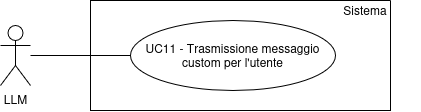
\includegraphics[width=0.7\linewidth]{UC11image.png}
    \caption{UC11 - Trasmissione messaggio custom per l'utente}
    \label{fig:UC11}
\end{figure}
\label{UC11}
\begin{itemize}
    \item \textbf{Attore$_G$ Principale:} LLM$_G$.
    \item \textbf{Precondizioni:} 
        \begin{itemize}
          \item Il Sistema$_G$ è operativo e accessibile.
        \end{itemize}
      \item \textbf{Postcondizioni:} L'LLM invia il messaggio custom generato al Sistema$_G$. Il Sistema$_G$ salva l'annuncio generato dall'LLM.
    \item \textbf{Scenario Principale:} 
        \begin{enumerate}
        \item L'LLM genera un annuncio basato sui dati precedentemente inviati;
        \item L'LLM invia al Sistema$_G$ il messaggio generato. 
        \end{enumerate}
    \item \textbf{User-Story$_G$ associata:} Come LLM$_G$ desidero trasmettere un messaggio custom, generato per un utente, al Sistema$_G$.
\end{itemize}
%%%%%%%%%%%%%%%%%%%%%%%%%%%%%%%%%%%%%%%%%%%%%%%%%%%%%%%%%%%%%%%%%%%%%%%%%%%


\newpage
\section{Requisiti$_G$}
%sicuramente da suddividere intenamente tra obbligatori, desiderabilli e opzionali

\subsection{Requisiti$_G$ funzionali}

% Definisci una nuova colonna centrata con larghezza fissa
\newcolumntype{C}[1]{>{\centering\arraybackslash}m{#1}}

\begin{center}
\renewcommand{\arraystretch}{1.5}
\begin{longtable}
{|>{\centering\arraybackslash}m{2.7cm}|>{\centering\arraybackslash}m{2.7cm}|>{\centering\arraybackslash}m{6cm}|>{\centering\arraybackslash}m{2.1cm}|}
%\begin{tabular}{|>{\vspace{5pt}}C{2.7cm}<{\vspace{5pt}}|>{\vspace{5pt}}C{2.7cm}<{\vspace{5pt}}|>{\vspace{5pt}}m{6cm}<{\vspace{5pt}}|>{\vspace{5pt}}C{2.1cm}<{\vspace{5pt}}|}
\hline
\textbf{Id. Requisito$_G$} & \textbf{Importanza} & \textbf{Descrizione} & \textbf{Fonti}\\
\endhead

\hline
 RF01 &  Obbligatorio &  L'utente privilegiato deve poter visualizzare la Dashboard$_G$ composta da una mappa interattiva con i vari Marker$_G$ su di essa. &  Capitolato$_G$, UC1\\
\hline
RF02 & Obbligatorio & L'utente privilegiato deve poter visualizzare dei Marker$_G$ che rappresentano i vari Percorsi$_G$ effettuati in tempo reale dagli utenti presenti nel Sistema$_G$ & Capitolato$_G$, UC1.1\\
\hline
RF03 & Obbligatorio & L'utente privilegiato deve poter visualizzare un Marker$_G$ che rappresenta un Percorso$_G$ effettuato in tempo reale da un utente presente nel Sistema$_G$ & Capitolato$_G$, UC1.1 e UC1.1.1\\
\hline
RF04 & Obbligatorio & L'utente privilegiato deve poter visualizzare tutti i punti di interesse riconosciuti dal Sistema$_G$. & Capitolato$_G$, UC1.2\\
\hline
RF05 & Obbligatorio & L'utente privilegiato deve poter visualizzare un Marker$_G$ che rappresenta un punto di interesse riconosciuto dal Sistema$_G$. & Capitolato$_G$, UC1.2 e UC1.2.1\\
\hline
RF06 & Obbligatorio & L'utente privilegiato deve poter visualizzare gli annunci pubblicitari provenienti da un determinato punto di interesse. & Capitolato$_G$, UC1.3\\
\hline
RF07 & Obbligatorio & L'utente privilegiato deve poter visualizzare un singolo annuncio pubblicitario tramite un Marker$_G$. & Capitolato$_G$, UC1.3 e UC1.3.1\\
\hline
RF08 & Obbligatorio & L'utente privilegiato deve poter visualizzare una Dashboard$_G$ relativa ad un singolo utente quando seleziona un Marker$_G$ utente nella Dashboard$_G$ principale. & Interna, UC3\\
\hline
RF09 & Obbligatorio & L'utente privilegiato deve poter visualizzare dei Marker$_G$ che rappresentano lo storico delle posizioni dell'utente a cui è riferita la Dashboard$_G$ di singolo utente. & Interna, UC3.1\\
\hline
RF10 & Obbligatorio & L'utente privilegiato deve poter visualizzare un Marker$_G$ che rappresenta la posizione dell'utente in un determinato istante nella Dashboard$_G$ di singolo utente. & Interna, UC3.1 e UC3.1.1\\
\hline
RF11 & Obbligatorio & L'utente privilegiato deve poter visualizzare, nella Dashboard$_G$ di singolo utente, tutti i punti di interesse riconosciuti dal Sistema$_G$. & Interna, UC3.2\\
\hline
RF12 & Obbligatorio & L'utente privilegiato deve poter visualizzare, nella Dashboard$_G$ di singolo utente, un Marker$_G$ che rappresenta un punto di interesse riconosciuto dal Sistema$_G$. & Interna, UC3.2 e UC3.2.1\\
\hline
RF13 & Obbligatorio & L'utente privilegiato deve poter visualizzare lo storico degli annunci pubblicitari generati per l'utente a cui è riferita la Dashboard$_G$ singolo utente. & Interna, UC3.3\\
\hline
RF14 & Obbligatorio & L'utente privilegiato deve poter visualizzare un singolo annuncio pubblicitario tramite un Marker$_G$ nella Dashboard$_G$ di singolo utente. & Interna, UC3.3 e UC3.3.1\\
\hline
RF15 & Obbligatorio & L'utente privilegiato deve poter visualizzare un pannello apposito contenente le informazioni dell'utente, a cui è riferita la Dashboard$_G$ di singolo utente, in forma tabellare. & Interna, UC3.4\\
\hline
RF16 & Obbligatorio & L'utente privilegiato deve poter visualizzare nel pannello apposito di visualizzazione informazioni dell'utente: il nome, il cognome, l'email, il genere, la data di nascita e lo stato civile. & Interna, UC3.4, UC3.4.1, UC3.4.2, UC3.4.3, UC3.4.4, UC3.4.5, UC3.4.6\\
\hline
RF17 & Obbligatorio & L'utente privilegiato deve poter visualizzare i dettagli del Marker$_G$ riguardante una singola posizione di un utente nella rispettiva Dashboard$_G$ & Interna, UC4\\
\hline
RF18 & Obbligatorio & L'utente privilegiato quando visualizza i dettagli del Marker$_G$, riguardante una singola posizione di un utente nella rispettiva Dashboard$_G$, deve poter vedere la latitudine, la longitudine e l'istante di rilevamento del Marker$_G$ & Interna, UC4, UC4.1, UC4.2 e UC4.3\\
\hline
RF19 & Opzionale & L'utente privilegiato deve poter visualizzare l'area di influenza di un punto di interesse selezionato. & Interna, UC5\\
\hline
RF20 & Obbligatorio & L'utente privilegiato deve poter visualizzare le informazioni dettagliate di un punto di interesse quando selezionato. & Interna, UC6\\
\hline
RF21 & Obbligatorio & L'utente privilegiato quando visualizza le informazioni dettagliate di un punto di interesse deve poter visualizzare la latitudine, la longitudine, il nome, la tipologia e la descrizione del punto di interesse. & Interna, UC6, UC6.1, UC6.2, UC6.3, UC6.4, UC6.5 e UC6.6\\
\hline
RF22 & Opzionale & L'utente deve poter visualizzare l'annuncio pubblicitario proveniente dal punto di interesse situato nell'area che sta attraversando. & Capitolato$_G$, UC2\\
\hline
RF23 & Obbligatorio & L'utente privilegiato deve poter visualizzare una tabella contenente le informazioni dei singoli PoI ordinati per la quantità di messaggi inviati nel mese. & Interna, UC7\\
\hline
RF24 & Obbligatorio & L'utente privilegiato deve poter visualizzare nella tabella dei PoI un singolo PoI, rappresentato da una riga della tabella. & Interna, UC7 e UC7.1\\
\hline
RF25 & Obbligatorio & L'utente privilegiato deve poter visualizzare in ogni riga della tabella dei PoI il nome, l'indirizzo, la tipologia (di che ambito si occupa), la descrizione e il numero di messaggi inviati durante il mese di un singolo PoI. & Interna, UC7, UC7.1, UC7.1.1, UC7.1.2, UC7.1.3, UC7.1.4 e UC7.1.5\\
\hline
RF26 & Obbligatorio & L'utente privilegiato deve poter visualizzare i dettagli di un annuncio generato. & Interna, UC8\\
\hline
RF27 & Obbligatorio & L'utente privilegiato quando visualizza i dettagli di un annuncio deve poter visualizzare la latitudine, la longitudine, l'istante di creazione, il nome dell'utente coinvolto, il nome del punto di interesse coinvolto e il contenuto dell'annuncio. & Interna, UC8, UC8.1, UC8.2, UC8.3, UC8.4, UC8.5 e UC8.6\\
\hline
RF28 & Obbligatorio & Il sensore deve essere in grado di trasmettere i dati rilevati in tempo reale al Sistema$_G$. & Capitolato$_G$, UC9\\
\hline
RF29 & Obbligatorio & Il sensore deve essere in grado di trasmettere il proprio id, la sua latitudine e longitudine al Sistema$_G$. & Interna, UC9, UC9.1, UC9.2 e UC9.3\\
\hline
RF30 & Obbligatorio & Il servizio LLM$_G$ deve essere in grado di ricevere i dati dell'utente e del punto di interesse inviati dal Sistema$_G$. & Interna, UC10\\
\hline
RF31 & Obbligatorio & Il servizio LLM$_G$ deve essere in grado di ricevere le informazioni dell'utente inviate dal Sistema$_G$, quali: il nome, il cognome, l'email, il genere, la data di nascita, lo stato civile e i suoi interessi. & Interna, UC10, UC10.1, UC10.1.1, UC10.1.2, UC10.1.3, UC10.1.4, UC10.1.5, UC10.1.6 e UC10.1.7\\
\hline
RF32 & Obbligatorio & Il servizio LLM$_G$ deve essere in grado di ricevere le informazioni del punto di interesse inviate dal Sistema$_G$, quali: il nome, l'indirizzo, la tipologia, la descrizione e la distanza del PoI dall'utente. & Interna, UC10, UC10.2, UC10.2.1, UC10.2.2, UC10.2.3, UC10.2.4 e UC10.2.5\\
\hline
RF33 & Obbligatorio & Il servizio LLM$_G$ deve essere in grado di trasmettere un messaggio custom, rappresentante il contenuto dell'annuncio per un utente, al Sistema$_G$. & Capitolato$_G$, UC11\\
\hline
\caption{Requisiti$_G$ funzionali}
\end{longtable}
\end{center}

%---------------------------------------------------------------------------------------------------------------------------------------------
\newpage
\subsection{Requisiti$_G$ di qualità}

\begin{table}[H]
\centering
\renewcommand{\arraystretch}{1.5}
\begin{tabular}{|>{\centering\arraybackslash}m{2.7cm}|>{\centering\arraybackslash}m{2.7cm}|>{\centering\arraybackslash}m{6cm}|>{\centering\arraybackslash}m{2.1cm}|}
%\begin{tabular}{|>{\vspace{5pt}}C{2.7cm}<{\vspace{5pt}}|>{\vspace{5pt}}C{2.7cm}<{\vspace{5pt}}|>{\vspace{5pt}}m{6cm}<{\vspace{5pt}}|>{\vspace{5pt}}C{2.1cm}<{\vspace{5pt}}|}
\hline
\textbf{Id. Requisito$_G$} & \textbf{Importanza} & \textbf{Descrizione} & \textbf{Fonti}\\
\hline
RQ01 & Obbligatorio & Presentare documento di Analisi-dei-Requisiti$_G$ contenente i diagrammi UML$_G$ relativi ai Casi-d'uso$_G$. & Capitolato$_G$\\
\hline
RQ02 & Obbligatorio & Devono essere rispettate tutte le Norme$_G$ definite nel documento \textit{Norme\_di\_Progetto\_v1.0.0.pdf}, nell'apposita sezione Analisi-dei-Requisiti$_G$. & Interna\\
\hline
RQ03 & Obbligatorio & Deve essere fornito il documento Specifica-Tecnica$_G$ riguardante le scelte di design del prodotto, con la motivazione delle scelte implementative e tecnologiche. & Capitolato$_G$, Verbale Esterno 2024-11-25\\
\hline
RQ04 & Obbligatorio & È necessaria la realizzazione di Test$_G$ che dimostrino il corretto funzionamento dei servizi e delle funzionalità previste, con una copertura minima dell'80\% e documentata tramite un report.  & Capitolato$_G$\\
\hline
RQ05 & Obbligatorio & È richiesto che il Sistema$_G$ venga testato in misura corrispondente ad almeno l'80\% della sua interezza (dal punto di vista di code, statement, branch e condition coverage) tramite Test$_G$ end-to-end, anche non automatizzati.  & Capitolato$_G$\\
\hline
RQ06 & Obbligatorio & I documenti di Analisi-dei-Requisiti$_G$ e Specifica-Tecnica$_G$ dovranno riguardare anche problemi aperti ed eventuali possibili soluzioni da approfondire in futuro.  & Capitolato$_G$\\
\hline
\end{tabular}
\caption{Requisiti$_G$ di qualità}
\end{table}

%---------------------------------------------------------------------------------------------------------------------------------------------
\newpage
\subsection{Requisiti$_G$ di vincolo}

\begin{table}[H]
\centering
\renewcommand{\arraystretch}{1.5}
\begin{tabular}{|>{\centering\arraybackslash}m{2.7cm}|>{\centering\arraybackslash}m{2.7cm}|>{\centering\arraybackslash}m{6cm}|>{\centering\arraybackslash}m{2.1cm}|}
%\begin{tabular}{|>{\vspace{5pt}}C{2.7cm}<{\vspace{5pt}}|>{\vspace{5pt}}C{2.7cm}<{\vspace{5pt}}|>{\vspace{5pt}}m{6cm}<{\vspace{5pt}}|>{\vspace{5pt}}C{2.1cm}<{\vspace{5pt}}|}
\hline
\textbf{Id. Requisito$_G$} & \textbf{Importanza} & \textbf{Descrizione} & \textbf{Fonti}\\
\hline
RV01 & Obbligatorio &  Per sviluppare il prodotto occorrerà utilizzare il linguaggio Python$_G$. & Interna\\
\hline 
RV02 & Obbligatorio & L'ambiente di sviluppo e di deployment deve utilizzare la tecnologia multi-container, in particolare docker$_G$ Compose. & Capitolato$_G$, Interna\\
\hline
RV03 & Obbligatorio & I rilevamenti dei sensori geoposizionali
devono essere memorizzati nel corretto formato in un time series Database$_G$, nel nostro Sistema$_G$ sarà ClickHouse$_G$. & Capitolato$_G$, Interna \\
\hline
RV04 & Obbligatorio & I dati raccolti e processati devono essere visualizzabili su una piattaforma di Dashboard$_G$ interattiva, come Grafana$_G$. & Capitolato$_G$, Interna\\
\hline
RV05 & Obbligatorio & Le coordinate generate per la simulazione di un utente che segue un Percorso$_G$ devono essere realistiche. & Capitolato$_G$\\
\hline
\end{tabular}

\caption{Requisiti$_G$ di vincolo}
\end{table}


%---------------------------------------------------------------------------------------------------------------------------------------------
\newpage
\subsection{Requisiti$_G$ prestazionali}

\begin{table}[H]
\centering
\renewcommand{\arraystretch}{1.5}
\begin{tabular}{|>{\centering\arraybackslash}m{2.7cm}|>{\centering\arraybackslash}m{2.7cm}|>{\centering\arraybackslash}m{6cm}|>{\centering\arraybackslash}m{2.1cm}|}
%\begin{tabular}{|>{\vspace{5pt}}C{2.7cm}<{\vspace{5pt}}|>{\vspace{5pt}}C{2.7cm}<{\vspace{5pt}}|>{\vspace{5pt}}m{6cm}<{\vspace{5pt}}|>{\vspace{5pt}}C{2.1cm}<{\vspace{5pt}}|}
\hline
\textbf{Id. Requisito$_G$} & \textbf{Importanza} & \textbf{Descrizione} & \textbf{Fonti}\\
\hline
RP01 & Obbligatorio &  Il Sistema$_G$ deve gestire inizialmente la generazione di un dato geoposizionale ogni 5 secondi e un utente noleggiatore del mezzo & Capitolato$_G$\\
\hline
RP02 & Obbligatorio &  Il Sistema$_G$ deve sopportare l'INSERT di una nuova posizione ogni 5 secondi per ogni utente e di un nuovo messaggio pubblicitario ogni 10 secondi per ogni utente  & Capitolato$_G$\\
\hline
\end{tabular}
\caption{Requisiti$_G$ prestazionali}
\end{table}

%---------------------------------------------------------------------------------------------------------------------------------------------


\newpage
\section{Tracciamento Requisiti$_G$}

\subsection{Fonte - Requisito}
\begin{center}
\begin{longtable}{|>{\vspace{5pt}}C{2.7cm}<{\vspace{5pt}}|>{\vspace{5pt}}C{2.7cm}<{\vspace{5pt}}|}
\hline
\textbf{Fonte} & \textbf{Id. Requisiti$_G$}\\
\hline
Capitolato$_G$ & RF01 \linebreak RF02 \linebreak RF03 \linebreak RF04 \linebreak RF05 \linebreak RF06 \linebreak RF07 \linebreak RF22 \linebreak RF28 \linebreak RF33 \linebreak RQ01  \linebreak RQ03 \linebreak RQ04 \linebreak RQ05 \linebreak RQ06 \linebreak RV02 \linebreak RV03 \linebreak RV04 \linebreak RV05 \linebreak RP01 \linebreak RP02\\
\hline
Interna & RF08 \linebreak RF09 \linebreak RF10 \linebreak RF11 \linebreak RF12 \linebreak RF13 \linebreak RF14 \linebreak RF15 \linebreak RF16 \linebreak RF17 \linebreak RF18 \linebreak RF19 \linebreak RF20 \linebreak RF21 \linebreak RF23 \linebreak RF24 \linebreak RF25 \linebreak RF26 \linebreak RF27 \linebreak RF29 \linebreak RF30 \linebreak RF31 \linebreak RF32 \linebreak RV01 \linebreak RV02 \linebreak RV03 \linebreak RV04 \linebreak RQ02 \\
\hline
UC1 & RF01\\
\hline
UC1.1 & RF02 \linebreak RF03\\
\hline
UC1.1.1 & RF03\\
\hline
UC1.2 & RF04 \linebreak RF05\\
\hline
UC1.2.1 & RF05\\
\hline
UC1.3 & RF06 \linebreak RF07\\
\hline
UC1.3.1 & RF07\\
\hline
UC3 & RF08\\
\hline
UC3.1 & RF09 \linebreak RF10\\
\hline
UC3.1.1 & RF10\\
\hline
UC3.2 & RF11 \linebreak RF12\\
\hline
UC3.2.1 & RF12\\
\hline
UC3.3 & RF13 \linebreak RF14\\
\hline
UC3.3.1 & RF14\\
\hline
UC3.4 & RF15 \linebreak RF16\\
\hline
UC3.4.1 & RF16\\
\hline
UC3.4.2 & RF16\\
\hline
UC3.4.3 & RF16\\
\hline
UC3.4.4 & RF16\\
\hline
UC3.4.5 & RF16\\
\hline
UC3.4.6 & RF16\\
\hline
UC4 & RF17 \linebreak RF18\\
\hline
UC4.1 & RF18\\
\hline
UC4.2 & RF18\\
\hline
UC4.3 & RF18\\
\hline
UC5 & RF19\\
\hline
UC6 & RF20 \linebreak RF21\\
\hline
UC6.1 & RF21\\
\hline
UC6.2 & RF21\\
\hline
UC6.3 & RF21\\
\hline
UC6.4 & RF21\\
\hline
UC6.5 & RF21\\
\hline
UC6.6 & RF21\\
\hline
UC2 & RF22\\
\hline
UC7 & RF23 \linebreak RF24 \linebreak RF25\\
\hline
UC7.1 & RF24 \linebreak RF25\\
\hline
UC7.1.1 & RF25\\
\hline
UC7.1.2 & RF25\\
\hline
UC7.1.3 & RF25\\
\hline
UC7.1.4 & RF25\\
\hline
UC7.1.5 & RF25\\
\hline
UC8 & RF26 \linebreak RF27\\
\hline
UC8.1 & RF27\\
\hline
UC8.2 & RF27\\
\hline
UC8.3 & RF27\\
\hline
UC8.4 & RF27\\
\hline
UC8.5 & RF27\\
\hline
UC8.6 & RF27\\
\hline
UC9 & RF28 \linebreak RF29\\
\hline
UC9.1 & RF29\\
\hline
UC9.2 & RF29\\
\hline
UC9.3 & RF29\\
\hline
UC10 & RF30 \linebreak RF31 \linebreak RF32\\
\hline
UC10.1 & RF31\\
\hline
UC10.1.1 & RF31\\
\hline
UC10.1.2 & RF31\\
\hline
UC10.1.3 & RF31\\
\hline
UC10.1.4 & RF31\\
\hline
UC10.1.5 & RF31\\
\hline
UC10.1.6 & RF31\\
\hline
UC10.1.7 & RF31\\
\hline
UC10.2.1 & RF32\\
\hline
UC10.2.2 & RF32\\
\hline
UC10.2.3 & RF32\\
\hline
UC10.2.4 & RF32\\
\hline
UC10.2.5 & RF32\\
\hline
UC11 & RF33\\
\hline
\caption{Tracciamento Fonte-Requisiti}
\end{longtable}
\end{center}

\subsection{Requisito - Fonte}
\begin{center}
\begin{longtable}{|>{\vspace{5pt}}C{2.7cm}<{\vspace{5pt}}|>{\vspace{5pt}}C{2.7cm}<{\vspace{5pt}}|}
\hline
\textbf{Requisito} & \textbf{Fonte}\\
\hline
RF01 & Capitolato$_G$, UC1\\
\hline
RF02 & Capitolato$_G$, UC1.1\\
\hline
RF03 & Capitolato$_G$, UC1.1 e UC1.1.1\\
\hline
RF04 & Capitolato$_G$, UC1.2\\
\hline
RF05 & Capitolato$_G$, UC1.2 e UC1.2.1\\
\hline
RF06 & Capitolato$_G$, UC1.3\\
\hline
RF07 & Capitolato$_G$, UC1.3 e UC1.3.1\\
\hline
RF08 & Interna, UC3\\
\hline
RF09 & Interna, UC3.1\\
\hline
RF10 & Interna, UC3.1 e UC3.1.1\\
\hline
RF11 & Interna, UC3.2\\
\hline
RF12 & Interna, UC3.2 e UC3.2.1\\
\hline
RF13 & Interna, UC3.3\\
\hline
RF14 & Interna, UC3.3 e UC3.3.1\\
\hline
RF15 & Interna, UC3.4\\
\hline
RF16 & Interna, UC3.4, UC3.4.1, UC3.4.2, UC3.4.3, UC3.4.4, UC3.4.5, UC3.4.6\\
\hline
RF17 & Interna, UC4\\
\hline
RF18 & Interna, UC4, UC4.1, UC4.2 e UC4.3\\
\hline
RF19 & Interna, UC5\\
\hline
RF20 & Interna, UC6\\
\hline
RF21 & Interna, UC6, UC6.1, UC6.2, UC6.3, UC6.4, UC6.5 e UC6.6\\
\hline
RF22 & Capitolato$_G$, UC2\\
\hline
RF23 & Interna, UC7\\
\hline
RF24 & Interna, UC7 e UC7.1\\
\hline
RF25 & Interna, UC7, UC7.1, UC7.1.1, UC7.1.2, UC7.1.3, UC7.1.4 e UC7.1.5\\
\hline
RF26 & Interna, UC8\\
\hline
RF27 & Interna, UC8, UC8.1, UC8.2, UC8.3, UC8.4, UC8.5 e UC8.6\\
\hline
RF28 & Capitolato$_G$, UC9\\
\hline
RF29 & Interna, UC9, UC9.1, UC9.2 e UC9.3\\
\hline
RF30 & Interna, UC10\\
\hline
RF31 & UC10, UC10.1, UC10.1.1, UC10.1.2, UC10.1.3, UC10.1.4, UC10.1.5, UC10.1.6 e UC10.1.7\\
\hline
RF32 & UC10, UC10.2, UC10.2.1, UC10.2.2, UC10.2.3, UC10.2.4 e UC10.2.5\\
\hline
RF33 & Capitolato$_G$, UC11\\
\hline
RQ01 & Capitolato$_G$\\
\hline
RQ02 & Interna\\
\hline
RQ03 & Capitolato$_G$\\
\hline
RQ04 & Capitolato$_G$\\
\hline
RQ05 & Capitolato$_G$\\
\hline
RQ06 & Capitolato$_G$\\
\hline
RV01 & Interna\\
\hline
RV02 & Capitolato$_G$, Interna\\
\hline
RV03 & Capitolato$_G$, Interna\\
\hline
RV04 & Capitolato$_G$, Interna\\
\hline
RV05 & Capitolato$_G$\\
\hline
RP01 & Capitolato$_G$\\
\hline
RP02 & Capitolato$_G$\\
\hline
\caption{Tracciamento Requisito-Fonte}
\end{longtable}
\end{center}

%---------------------------------------------------------------------------------------------------------------------------------------------

\subsection{Riepilogo}
\begin{table}[H]
\centering
\begin{tabular}{|>{\vspace{4pt}}C{2.4cm}<{\vspace{4pt}}|>{\vspace{4pt}}C{2.3cm}<{\vspace{4pt}}|>{\vspace{4pt}}C{2.3cm}<{\vspace{4pt}}|>{\vspace{4pt}}C{2.3cm}<{\vspace{4pt}}|>{\vspace{4pt}}C{1.4cm}<{\vspace{4pt}}|}
\hline
\textbf{Tipologia} & \textbf{Obbligatori} & \textbf{Desiderabili} & \textbf{Opzionali} & \textbf{Totale}\\
\hline
Funzionali & 31 & - & 2 & 33\\
\hline
Di qualità & 6 & - & - & 6 \\
\hline
Di vincolo & 5 & - & - & 5 \\
\hline
Prestazionali & 2 & - & - & 2 \\
\hline
Totale & 44 & - & 2 & 46 \\
\hline
\end{tabular}
\caption{Riepilogo}
\end{table}

\end{justify}
\end{document}
